\begin{introduction}
    \item 距离空间~\ref{def:Metric}
    \item 距离空间的点集~\ref{pointset}
    \item 距离空间的完备性~\ref{complete}
    \item $Baire$定理~\ref{the:Baire}
    \item 压缩映射定理~\ref{zip}
    \item 拓扑空间~\ref{topo}
    \item 距离空间上的紧集~\ref{compact}
    \item $Arzela-Ascoli$定理~\ref{the:AA}
  \end{introduction}
\section{距离空间 $Metric \ Space$}
\subsection{定义及举例}
事实上,我们可以通过定义距离这个几何上的概念很好地定义收敛和连续这两个我们关心的分析上的概念。
例如,在欧氏空间$\mathbb{R}^n$上,我们定义距离:
\[\mathbb{R}^n=\{\overrightarrow{x}=(x_1,x_2,\cdots,x_n)|x_i \in \mathbb{R} \ (i=1,2,\cdots,n)\}\]
\[d(\overrightarrow{x},\overrightarrow{y})=\sqrt{\sum_{i=1}^n\left|x_i-y_i\right|^2}\]
\paragraph*{收敛性} \quad $\overrightarrow{x}_m \rightarrow \overrightarrow{x}$:
\[\overrightarrow{x}_m \rightarrow \overrightarrow{x} \Leftrightarrow d(\overrightarrow{x},\overrightarrow{y}) \rightarrow 0 \Leftrightarrow x_{m,i} \rightarrow x_i \ (i=1,2,\cdots,n)\]
\paragraph*{连续性} \quad 定义函数$f$:
\[f:\mathbb{R}^n \rightarrow \mathbb{R}^m\]
如果$f$满足
\[\overrightarrow{x}_0 \in \mathbb{R}^n\ , \ \forall \varepsilon >0 \ , \ \exists \, \delta >0 \ , \quad s.t. \quad d_{\mathbb{R}^n}(\overrightarrow{x},\overrightarrow{x}_0)<\delta \ , \ d_{\mathbb{R}^m}(f(\overrightarrow{x}),f(\overrightarrow{x}_0))<\varepsilon\]
则称$f$在点$\overrightarrow{x}_0$连续,进而可以推广到处处连续。

从欧氏空间出发,我们可以定义抽象距离空间:
\begin{definition}[抽象距离空间] \label{def:Metric}
    $X$是一个非空集合,$d$是一个定义在$X \times X$上的函数,满足:\\
    1、非负性:$d(x,y) \geq 0$且$d(x,y)=0$当且仅当$x=y$;\\
    2、对称性:$d(x,y)=d(y,x)$;\\
    3、三角不等式:$d(x,y) \leq d(x,z)+d(z,y)$
\end{definition}

下面我们看几个距离空间的例子:
\paragraph*{例1} \quad $C[a,b]$,定义距离
\[d(x(t),y(t))=\mathop{\text{sup}}\limits_{t \in [a,b]}\left|x(t)-y(t)\right|\]
前两个性质显然成立,主要证第三条:

由于由三角不等式恒成立:
\[\left|x(t)-y(t)\right| \leq \left|x(t)-z(t)\right|+\left|z(t)-y(t)\right|\]
两边取上确界即证毕:
\[\mathop{\text{sup}}\limits_{t \in [a,b]}\left|x(t)-y(t)\right| \leq \mathop{\text{sup}}\limits_{t \in [a,b]}\left|x(t)-z(t)\right|+\mathop{\text{sup}}\limits_{t \in [a,b]}\left|z(t)-y(t)\right|\]
\[d(x,y) \leq d(x,z)+d(z,y)\]

\paragraph*{例2} \quad 空间$s=\{x=\{\xi_i\}_{i=1}^{+\infty} \ , \ \xi_i \in \mathbb{R}\}$(规定后续符号对应:$x,t,z \rightarrow \xi,\eta,\psi$),定义距离
\[d(x,y)=\sum_{i=1}^{+\infty}\frac{1}{2^i}\frac{|\xi_i-\eta_i|}{1+|\xi_i-\eta_i|}\]
同样,前两条性质显然,下证第三条:

同样由三角不等式:
\[\left|\xi_i-\eta_i\right| \leq \left|\xi_i-\psi_i\right|+\left|\psi_i-\eta_i\right|\]
\[\sum_{i=1}^{+\infty}\frac{1}{2^i}\frac{|\xi_i-\eta_i|}{1+|\xi_i-\eta_i|} \leq \sum_{i=1}^{+\infty}\frac{1}{2^i}\frac{\left|\xi_i-\psi_i\right|+\left|\psi_i-\eta_i\right|}{1+\left|\xi_i-\psi_i\right|+\left|\psi_i-\eta_i\right|}\]
\[=\sum_{i=1}^{+\infty}\frac{1}{2^i}\frac{\left|\xi_i-\psi_i\right|}{1+\left|\xi_i-\psi_i\right|+\left|\psi_i-\eta_i\right|}+\sum_{i=1}^{+\infty}\frac{1}{2^i}\frac{\left|\psi_i-\eta_i\right|}{1+\left|\xi_i-\psi_i\right|+\left|\psi_i-\eta_i\right|}\]
\[\leq \sum_{i=1}^{+\infty}\frac{1}{2^i}\frac{\left|\xi_i-\psi_i\right|}{1+\left|\xi_i-\psi_i\right|}+\sum_{i=1}^{+\infty}\frac{1}{2^i}\frac{\left|\psi_i-\eta_i\right|}{1+\left|\psi_i-\eta_i\right|}=d(x,z)+d(z,y)\]

\paragraph*{例3} \quad 空间$S(E) \ E \subseteq \mathbb{R}$是$E$上$Lebesgue$可积函数全体,定义距离
\[d(x,y)=\int_E\frac{\left|x(t)-y(t)\right|}{1+\left|x(t)-y(t)\right|}dt\]

证明类似例2。

顺便一说,在这个距离定义下的收敛等价于依测度收敛,下一小节会证明。

\paragraph*{例4} \quad 空间$L^2(E)=\{f\text{在$E$上可测} \ , \ \int_E|f|^2<+\infty\}$上,我们定义距离
\[d(x,y)=\sqrt{\int_E|x(t)-y(t)|^2dt}\]
同样,前两条性质显然,下证第三条:

\[d^2(x,y)=\int_E|x(t)-y(t)|^2dt=\int_E(x^2(t)+y^2(t)-2x(t)y(t))dt\]
\[\leq \int_Ex^2(t)dt+\int_Ey^2(t)dt+2\int_E|x(t)||y(t)|dt \leq \int_Ex^2(t)dt+\int_Ey^2(t)dt+2\sqrt{\int_Ex^2(t)dt}\sqrt{\int_Ey^2(t)dt}\]
\[\leq \left(\sqrt{\int_Ex^2(t)dt}+\sqrt{\int_Ey^2(t)dt}\right)^2\]
此时,如果我们令$x=f-h \ , \ y=g-h$,则上式可改写为
\[d^2(f,g) \leq (d(f,h)+d(g,h))^2\]
原不等式即证。

欧氏空间是距离空间也可类似证明。

上面的几个例子都是函数空间,当然我们也可以来看几个不是函数空间的距离空间的例子。

\paragraph*{例5} \quad 离散空间$X$为任意集合,定义距离
\[d(x,y)=\left \{
\begin{array}{c}
1 \ , \ x \neq y \\ 0 \ , \ x=y
\end{array}   
\right .
\]

\paragraph*{例6} \quad 图($Graph$)

图包含顶点集$V=\{v_1,v_2,\cdots,v_n\}$,边集$E=\{e_{ij}\}$,定义$d(v_i,v_j)$为$v_i$和$v_j$之间最短的路线长度。

\subsection{距离空间的性质}
在上一小节我们介绍了距离空间以及距离的概念,我们可以很自然地引入一般度量意义下的收敛。

\paragraph*{距离空间$(X,d)$上的收敛} \quad 我们称$x_n$收敛于$x$,当其满足
\[\lim_{n \rightarrow \infty}d(x_n,x)=0\]

这里我们回顾一下之前接触过的函数列收敛的种类。

\paragraph*{逐点收敛} \quad $f_n(x) \rightarrow f(x) \ , \ x \in [a,b] \ , \ (n \rightarrow \infty)$
\[\forall x \in [a,b] \ , \ \forall \varepsilon>0 \ , \ \exists \, N(\varepsilon,x)>0 \ , \quad s.t. \quad n \geq N \ , \ |f_n(x)-f(x)|<\varepsilon\]

\paragraph*{一致收敛} \quad $f_n(x) \rightrightarrows f(x) \ , \ (n \rightarrow \infty)$
\[\forall x \in [a,b] \ , \ \forall \varepsilon>0 \ , \ \exists \, N(\varepsilon)>0 \ , \quad s.t. \quad n \geq N \ , \ |f_n(x)-f(x)|<\varepsilon\]

\paragraph*{依测度收敛} \quad $f_n(x) \rightarrow f(x)\textbf{ in measure} \ , \ (n \rightarrow \infty)$
\[\forall \sigma>0 \ , \ \lim_{n \rightarrow \infty}m\{|f_n(x)-f(x)| \geq \sigma\}=0\]

逐点收敛和一致收敛的区别仅在$N$是否与$x$有关,现在我们来考察一下这些收敛跟距离的关系。
我们知道距离这个概念能诱导出收敛,但是收敛并不意味着一定有距离意义。很显然,逐点收敛没有对应的距离意义,因为$N$与$x$有关。

下面我们来看其他两种收敛对应的距离空间上的收敛。

\paragraph*{例1} \quad $X=C[a,b]$
\[d(x(t),y(t))=\mathop {\text{sup}}\limits_{t \in [a,b]}|x(t)-y(t)|\]
\[x_n(t) \rightarrow x(t) \quad (n \rightarrow \infty) \qquad \lim_{n \rightarrow \infty}d(x_n(t),x)=\lim_{n \rightarrow \infty}\mathop {\text{sup}}\limits_{t \in [a,b]}|x_n(t)-x(t)|=0\]
\[\forall \varepsilon>0 \ , \ \exists \, N(\varepsilon)>0 \ , \quad s.t. \quad n \geq N \ , \ \mathop {\text{sup}}\limits_{t \in [a,b]}|x_n(t)-x(t)|<\varepsilon\]
即
\[\forall t \in [a,b] \ , \ \forall \varepsilon>0 \ , \ \exists \, N(\varepsilon)>0 \ , \quad s.t. \quad n \geq N \ , \ |x_n(t)-x(t)|<\varepsilon\]
可见该空间下距离的收敛等价于一致收敛。

\paragraph*{例2} \quad 空间$S(E) \ E \subseteq \mathbb{R}$是$E$上$Lebesgue$可积函数全体
\[d(x,y)=\int_E\frac{\left|x(t)-y(t)\right|}{1+\left|x(t)-y(t)\right|}dt\]
证明:Part 1
\[\lim_{n \rightarrow \infty}d(x_n(t),x(t))=\lim_{n \rightarrow \infty}\int_E\frac{\left|x_n(t)-x(t)\right|}{1+\left|x_n(t)-x(t)\right|}dt=0\]
记$M=\{|x_n(t)-x(t)| \geq \sigma\}\cap E$
\[\int_E\frac{\left|x_n(t)-x(t)\right|}{1+\left|x_n(t)-x(t)\right|}dt \geq \int_M\frac{\left|x_n(t)-x(t)\right|}{1+\left|x_n(t)-x(t)\right|}dt \geq \int_M\frac{\sigma}{1+\sigma}dt=\frac{\sigma}{1+\sigma}m(M)\]
则有
\[0 \leq m(M) \leq \frac{1+\sigma}{\sigma}d(x_n(t),x(t))\rightarrow 0 \quad n \rightarrow \infty\]
于是有
\[f_n(x) \rightarrow f(x)\textbf{ in measure} \ , \ (n \rightarrow \infty)\]
Part 2
\[\int_E\frac{\left|x_n(t)-x(t)\right|}{1+\left|x_n(t)-x(t)\right|}dt=\int_M\frac{\left|x_n(t)-x(t)\right|}{1+\left|x_n(t)-x(t)\right|}dt+\int_{E-M}\frac{\left|x_n(t)-x(t)\right|}{1+\left|x_n(t)-x(t)\right|}dt\]
\[\leq m(M)+\frac{\sigma}{1+\sigma}m(E-M) \leq m(M)+\frac{\sigma}{1+\sigma}m(E)\]
\[\forall \varepsilon>0 \ , \ let \ \sigma=\frac{\varepsilon}{m(E)} \ (assume \ m(E)>1) \ , \ \exists \, N>0 \quad s.t. \quad n \geq N \ , \ m(M)<\varepsilon\]
\[d(x_n(t),x(t)) \leq \varepsilon+\frac{\varepsilon}{1+\sigma}<2\varepsilon\]
\[\lim_{n \rightarrow \infty}d(x_n(t),x(t))=0\]
证毕。

距离空间还有其他的性质如下:

1) 极限存在必定唯一;

2) $x_n \rightarrow x$,则$\{x_{n,i}\} \subset \{x_n\} \quad s.t. \quad x_{n,i} \rightarrow x$ (距离意义下的收敛)

3) $x_n \rightarrow x$,$x_n \rightarrow x$,则有$d(x_n,y_n) \rightarrow d(x,y)$

前两个性质容易得到,我们下证第三条。

由三角不等式
\[d(x_n,y_n) \leq d(x_n,x)+d(x,y)+d(y,y_n) \Leftrightarrow d(x_n,y_n)-d(x,y) \leq d(x_n,x)+d(y_n,y)\]
\[d(x,y) \leq d(x,x_n)+d(x_n,y_n)+d(y_n,y) \Leftrightarrow d(x_n,y_n)-d(x,y) \geq d(x_n,x)+d(y_n,y)\]
\[\Rightarrow \ |d(x_n,y_n)-d(x,y)|=d(x_n,x)+d(y_n,y) \ \rightarrow 0 \ (n \rightarrow \infty)\]
证毕。

我们也可以定义一般度量意义下的连续性。
\paragraph*{距离空间$(X,d)$上的连续} \quad 设$f:(X,d_X) \rightarrow (Y,d_Y)$是距离空间中的映射。我们称$f$在$x_0$处连续,如果其满足
\[\forall x_0 \in X \ , \ \forall \varepsilon>0 \ , \ \exists \, \delta>0 \ , \quad s.t. \quad d_Y(f(x),f(x_0))<\varepsilon \ , \ if \ d_X(x,x_0)<\delta\]

定义了单点连续后我们容易得到如果$f$在任意$x_0 \in X$上都连续我们就称$f$在$X$上连续。

还有一个比较值得探讨的东西是等距映射。
\paragraph*{等距映射} \quad 设$f:(X,d_X) \rightarrow (Y,d_Y)$是距离空间中的映射,若满足
\[\forall x,y \in X \ , \ d_Y(f(x),f(y))=d_X(x,y)\]
则称$f$为等距映射,称$(X,d_X)$与$(Y,d_Y)$等距($isometry$)。

显然,等距映射是连续且单射的,且$x \rightarrow f(x)$是双射。

举个例子,$\mathbb{R}^n \rightarrow \mathbb{R}^n$的等距映射有且仅有合同变换一种。
\[f(\overrightarrow{x})=A\overrightarrow{x}+\overrightarrow{x}_0 \quad A \in O(n)(\text{正交矩阵})\]

\subsection{距离空间的点集} \label{pointset}
这一小节主要是想说明一般度量空间内的如下几个定义:开集、内部、闭集、闭包、稠密性、可分性。这些概念在拓扑学中有更广泛的定义。

首先我们想在度量空间内定义开集,我们首先需要定义开球:
\begin{definition}[开球]
    我们称$B_r(x)=S(x,r)=\{y \in X \ , \ d(x,y)<r\}$为以$x$为球心$r$为半径的开球。
\end{definition}
\begin{definition}[开集]
    设$A \subset X$,如果$A$满足
    \[\forall x \in A \ , \ \exists \, \varepsilon>0 \quad s.t. \quad B_{\varepsilon}(x) \subset A\]
    则称$A$为$X$中的开集。
\end{definition}
进而,我们还能定义内点和内部。
\begin{definition}[内点]
    设$A \subset X$是开集,若
    \[x \in X \ , \ \exists \, \varepsilon>0 \quad s.t. \quad B_{\varepsilon}(x) \subset A\]
    则称$x$是$A$的内点。
\end{definition}
\begin{definition}[内部]
    $A$的全部内点构成的集合称为$A$的内部,记作\AA。
\end{definition}
容易看出$A$是开集$ \ \Leftrightarrow \ A=$\AA。

下面我们来看看开集的基本性质。
\begin{theorem}
    设$(X,d)$是距离空间,则有:\\
    1、$X$,$\varnothing$是开集;\\
    2、任意多个开集的并是开集;\\
    3、有限多个开集的交是开集。
\end{theorem}

前两个性质是显然的,下面我们来看看第三个性质的证明。

假设$G_i \ (i=1,2,\cdots,k)$都是开集。
\[\bigcap_{i=1}^kG_i \neq \varnothing \ \Leftrightarrow \ x \in \bigcap_{i=1}^kG_i \ and \ \exists \, \varepsilon_i >0 \ , \ B_{\varepsilon_i}(x) \subset G_i \quad (i=1,2,\cdots,k)\]
则,我们可以取
\[\varepsilon=\text{min}\{\varepsilon_1,\varepsilon_2,\cdots,\varepsilon_k\} \tag{2-1}\]
使得
\[B_{\varepsilon}(x) \subset B_{\varepsilon_i}(x) \subset G_i \qquad (i=1,2,\cdots,k)\]
即
\[B_{\varepsilon}(x) \subset \bigcap_{i=1}^kG_i\]
证毕。

为什么必须是有限个开集的交?从2-1式我们应该能看出来。
如果是取无限个开集的交,2-1式中的min将无法取到,而应取inf,而取inf的后果将有可能使得$\varepsilon=0$,让后续证明失效。
\begin{definition}[接触点]
    设$A \subset X$是开集,若
    \[x \in X \ , \ \forall \varepsilon>0 \quad s.t. \quad B_{\varepsilon}(x) \cap A \neq \varnothing\]
    则称$x$是$A$的接触点。
\end{definition}

当$x \in A$时,$x$一定是$A$的接触点,$A$的接触点不一定属于$A$。

\begin{definition}[闭包]
    $A$的全部接触点构成的集合称为$A$的闭包,记作$\bar{A}$。
\end{definition}
\begin{definition}[闭集]
    定义1:若$A=\bar{A}$则称$A$为闭集。\\
    定义2:若$A^c$为开集,则$A$为闭集。
\end{definition}

下面我们来看看闭包的性质。
\begin{theorem}
    设$(X,d)$是距离空间,$A,B \subset X$,则有
    \[1)\bar{\varnothing}=\varnothing \, ; \quad 2)A \subset \bar{A} \, ; \quad 3)\bar{\bar{A}}=\bar{A} \, ; \quad 4)\overline{A \cup B}=\bar{A} \cup \bar{B}\]
\end{theorem}

前两点是显然的,我们来证明一下第三第四点。

Proof (2):设
\[x \in \bar{\bar{A}} \ , \ \forall \varepsilon>0 \ , \ B_{\varepsilon}(x) \cap \bar{A} \neq \varnothing\]
\[\Rightarrow \ \exists \, y \in B_{\varepsilon}(x) \cap \bar{A} \ \Rightarrow \ B_{\varepsilon}(y) \cap A \neq \varnothing \ \Rightarrow \ B_{\varepsilon}(y) \subset B_{2\varepsilon}(x) \ \Rightarrow \ B_{2\varepsilon}(x) \cap A \neq \varnothing \ \Rightarrow \ x \in \bar{A}\]

Proof (3):设$x \in \overline{A \cup B}$
\[\forall \varepsilon>0 \ , \ B_{\varepsilon}(x) \cap (A \cup B) \neq \varnothing \ \Rightarrow \ B_{\varepsilon}(x) \cap A \neq \varnothing \ or \ B_{\varepsilon}(x) \cap B \neq \varnothing\]
假设$x \notin \bar{A} \cup \bar{B}$则
\[\exists \, \varepsilon_1,\varepsilon_2>0 \quad s.t. \quad B_{\varepsilon_1}(x) \cap A=\varnothing \ , \ B_{\varepsilon_2}(x) \cap B=\varnothing\]
\[\varepsilon:=\text{min}\{\varepsilon_1,\varepsilon_2\} \ s.t. B_{\varepsilon_1}(x) \cap A=\varnothing \ and \ B_{\varepsilon_2}(x) \cap B=\varnothing\]
矛盾,故$x \in \bar{A} \cup \bar{B}$。

反之,设$x \in \bar{A} \cup \bar{B}$,不妨设$x \in A$,
\[\forall \varepsilon>0 \ , \ B_{\varepsilon}(x) \cap A \neq \varnothing \ \Rightarrow \ \forall \varepsilon>0 \ , \ B_{\varepsilon}(x) \cap (A \cup B) \neq \varnothing \ \Rightarrow  \ x \in \overline{A \cup B}\]
证毕。

下面我们来看闭集的一些性质。
\begin{theorem}
    设$(X,d)$是距离空间,则有:\\
    1、$X$,$\varnothing$是闭集;\\
    2、任意多个闭集的交是闭集;\\
    3、有限多个闭集的并是闭集。
\end{theorem}

这些性质的证明可以通过$De \ Morgan's \ Law$证明类似例2。
\begin{theorem}[$De \ Morgan's \ Law$]
\[\left(\bigcup\limits_{\lambda \in \Lambda}A_{\lambda}\right)^c=\bigcap\limits_{\lambda \in \Lambda}A_{\lambda}^c \qquad \left(\bigcap\limits_{\lambda \in \Lambda}A_{\lambda}\right)^c=\bigcup\limits_{\lambda \in \Lambda}A_{\lambda}^c\]
\end{theorem}

闭集还有如下性质,同时它也是闭集的另一种定义方式:
\begin{theorem}
    设$(X,d)$是距离空间,$A$为闭集,$\{x_n\} \in A$,若$x_n \rightarrow x$,则$x \in A$。
\end{theorem}

下面我们来看稠密性和可分性。

\paragraph*{例1} \quad $\mathbb{R}$中,$\mathbb{Q}$是稠密的($\mathbb{R}$上任意小的区间都有$x \in \mathbb{Q}$);$\mathbb{Q}$是可数的。
\begin{definition}[稠密性]
    若$A \subset X$且$\bar{A}=X$则称$A$在$X$中是稠密的(原本应该是$X \subseteq \bar{A}$,当$X$取全空间的时候只能是$\bar{A}=X$)。
\end{definition}
\begin{definition}[可分性]
    若$X$有可数的稠密子集则称$X$是可分的。
\end{definition}
\paragraph*{例2} \quad $C[a,b]$是可分的

\textbf{Proof:}利用$Weierstrass$定理
\begin{theorem}[$Weierstrass$定理]
    设$f(x)$是$[a,b]$上的连续函数,那么存在一列多项式$\{P_n(x)\}$,使得
    \[P_n(x) \rightrightarrows f(x) \quad (n \rightarrow \infty)\]
\end{theorem}
$\forall P_n(x)$,存在有理多项式列$\{q_{n,i}(x)\}_{i=1}^{\infty}$使得$q_{n,i}(x) \rightrightarrows P_n(x) \ (i \rightarrow \infty)$,则
\[\forall k \in \mathbb{N}_+ \ , \ \exists \, n_k,i_k \ , \ q_{n_k,i_k}(x) \rightrightarrows f(x)\]
再多证明一步即可:
\[d(q_{n_k,i_k}(t),f(t)) \rightarrow 0 \ (n \rightarrow \infty) \ \Leftrightarrow \ q_{n_k,i_k}(x) \rightrightarrows f(x) \tag{*}\]
Proof (*):
\[\forall k \in \mathbb{Z}_+ \ , \ \exists \, n_k>0 \quad s.t. \quad n \geq n_k \ , \ |P_n(t)-f(t)|<\frac{1}{k} \ , \ \forall t \in [a,b]\]
\[\exists \, i_k>0 \ , \quad s.t. \quad i \geq i_k \ , \ |q_{n_k,i_k}(t)-P_{n_k}(t)|<\frac{1}{k} \ , \ \forall t \in [a,b]\]
\[|q_{n_k,i_k}(t)-f(t)| \leq |q_{n_k,i_k}(t)-P_{n_k}(t)|+|P_n(t)-f(t)|<\frac{1}{k}+\frac{1}{k}=\frac{2}{k} \ , \ \forall t \in [a,b]\]
上述是要证的两个条件的共同$\varepsilon-\delta$语言的描述,故(*)证毕。

对上述证明做一下形象化证明,上述的证明实质上是相当于取一个对角线子列$\{a_{i,j}\}$:
\[
\begin{array}{cccccc}
    a_{1,1} & a_{1,2} & a_{1,3} & \cdots & \rightarrow & a_1 \\
    a_{2,1} & a_{2,2} & a_{2,3} & \cdots & \rightarrow & a_2 \\
    \vdots & \vdots & \vdots & \vdots & \rightarrow & \vdots \\
      &   &   &   &   & \downarrow \\
    \vdots & \vdots & \vdots & \vdots & \rightarrow & a_{\infty}
\end{array}    
\]

\paragraph*{例2} \quad $l^{\infty}=\{x|\left\{\xi_i\right\}_{i=1}^{\infty} \ (\xi_i \in \mathbb{R}) \ , \ d(x,0)<\infty\}$,$x$为实数列且$l^{\infty} \in \{\text{所有实数列}\}$,定义$l^{\infty}$上的距离:
\[d(x,y)=\mathop {\text{sup}}\limits_{i=1,2,\cdots}|x_i-y_i| \qquad let \ x=\left\{x_i\right\}_{i=1}^{\infty} \ , \ y=\left\{y_i\right\}_{i=1}^{\infty}\]
是不可分的。

其中有
\[d(x,0)<\infty \Leftrightarrow \mathop {\text{sup}}\limits_{i=1,2,\cdots}|\xi_i|<\infty\]

\textbf{Proof:}易知有:
\[D=\{\left\{\xi_i\right\}_{i=1}^{\infty} \ , \ \xi_i=0 \ or \ 1\} \quad \forall x,y \in D \ , \ d(x,y)=0 \ or \ 1\]
显然,如果我们把$D$中的每一位放到$0.$后面,可以看出就是一个$[0,1]$区间上的二进制表示,故$D$的基数与$\mathbb{R}$相同。
\[card(D)=card([0,1])=card(\mathbb{R})\]

我们利用反证法,假设$l^{\infty}$是可分的,则其可以表示为一个可数稠密子集的闭包
\[l^{\infty}=\bar{A}\]
由于$A$稠密且可数,我们可以知道
\[l^{\infty} \in \bigcup_{a \in A}B_{\frac{1}{3}}(a) \tag{*}\]
(Proof(*): 
\[\forall x \in l^{\infty} \ , \ l^{\infty}=\bar{A} \ \Rightarrow \ x\text{是}A\text{的接触点} \ \Rightarrow \ B_{\frac{1}{4}}(x)\cap A \neq \varnothing\]
\[let \ y \in B_{\frac{1}{4}}(x)\cap A \ \Rightarrow \ x \in B_{\frac{1}{3}}(y) \ \Rightarrow \ x \in \bigcup_{a \in A}B_{\frac{1}{3}}(a)\]
\textbf{Q.E.D.})
\begin{figure}[htbp]
    \center
    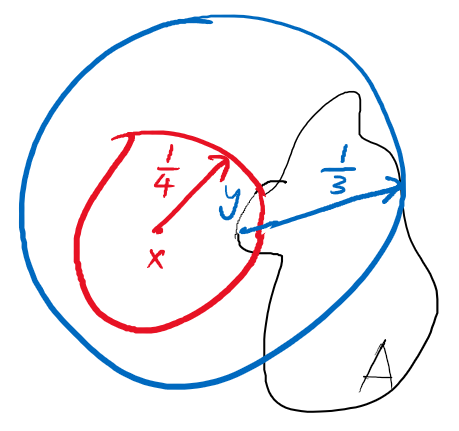
\includegraphics[scale=0.5]{./fig/2.1.3_1.png}
\end{figure}

$A$可数,$D$不可数,且有$D \in l^{\infty} \in \bigcup_{a \in A}B_{\frac{1}{3}}(a)$:
\[\Rightarrow \ \exists \, x \neq y \ , \ x,y \in D \ , \quad s.t. \quad x,y \in \bigcup_{a \in A}B_{\frac{1}{3}}(a) \ (a \in A)\]
\[\Rightarrow \ d(x,y)=1 \leq d(x,a)+d(y,a) \leq \frac{2}{3} \qquad \text{矛盾}\]
故$l^{\infty}$不可分。

\subsection{距离空间的完备性}\label{complete}
\begin{definition}[柯西列]
    设$(X,d)$是距离空间,若$X$中的点列$\{x_n\}_{n=1}^{\infty}$满足:
    \[\{x_n\}_{n=1}^{\infty} \in X \ , \ \forall \varepsilon>0 \ , \ \exists \, N>0 \ , \quad s.t. \quad n,m \geq N \ , \ d(x_n,x_m)<\varepsilon\]
    则称$\{x_n\}_{n=1}^{\infty}$为柯西列。
\end{definition}

\paragraph*{例1} \quad 收敛点列一定是柯西列,柯西列是否一定收敛?

$\mathbb{R}^n$中是,一般距离空间不成立。
\begin{definition}[完备距离空间]
    设$(X,d)$是距离空间。若该距离空间中所有柯西列都收敛,则称距离空间$(X,d)$是完备的。
\end{definition}

\paragraph*{例2} \quad $S=(C[0,1],d_1) \quad d_1(x,y)=\int_0^1|x(t)-y(t)|dt$这个距离空间是不完备的。

找反例,令
\[x_n(t)=\left \{
\begin{array}{ll}
    0 & ,t \in [0,\frac{1}{2}-\frac{1}{n}) \\
    \frac{n}{2}x-\frac{n}{4}+\frac{1}{2} & ,t \in [\frac{1}{2}-\frac{1}{n},\frac{1}{2}+\frac{1}{n}] \\
    1 & ,t \in (\frac{1}{2}+\frac{1}{n},1]
\end{array}
\right .\]
\begin{figure}[htbp]
    \center
    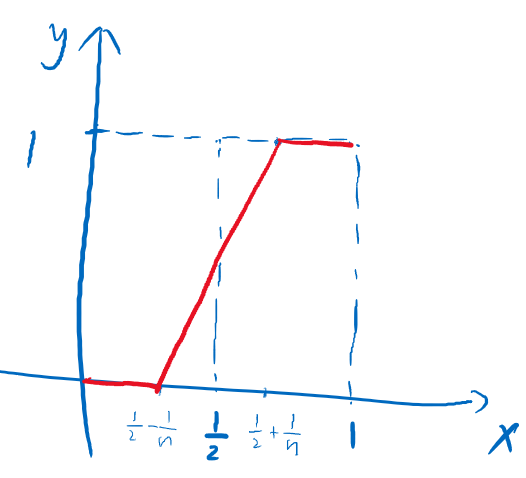
\includegraphics[scale=0.4]{./fig/2.1.4_1.png}
    \caption{$x_n(t)$的图像}
\end{figure}
\[m>n \ , \ d_1(x_n,x_m)=\int_0^1|x_n(t)-x_m(t)|dt \leq \int_{\frac{1}{2}-\frac{1}{n}}^{\frac{1}{2}+\frac{1}{n}}|x_n(t)-x_m(t)|dt \leq \frac{2}{n} \cdot 1=\frac{2}{n}\]
\[\forall \varepsilon>0 \ , \ let \ N>\frac{2}{\varepsilon} \ , \ s.t. m>n \geq N \ d_1(x_m,x_n) \leq \frac{2}{n} < \varepsilon\]
$\{x_n(t)\}$是柯西列。且可以看出$x_n(t)$是逐点收敛(先固定t)于下列函数$x_{\infty}(t)$。
\[x_n(t) \rightarrow x_{\infty}(t)=\left \{
\begin{array}{ll}
    0 & ,t \in [0,\frac{1}{2}) \\
    \frac{1}{2} & ,t=\frac{1}{2} \\
    1 & ,t \in (\frac{1}{2},1]
\end{array}
\right . \qquad (n \rightarrow \infty)\]

采用反证法,假设
\[y \in S \quad s.t. \quad d_1(x_n,y) \rightarrow 0 \ (n \rightarrow \infty) \ \Leftrightarrow \ \int_0^1|x_n(t)-y(t)|dt \rightarrow 0 \ (n \rightarrow \infty)\]
则有
\[d_1(x_{\infty},y) \leq d_1(x_{\infty},x_n)+d_1(x_n,y) \rightarrow 0 \ \Rightarrow \ x_{\infty}(t)=y(t)\]
由$y \in S \ \Rightarrow \ y \in C[0,1]$可得矛盾。

故上述函数列$\{x_n(t)\}$并不在距离空间$(S,d_1)$中收敛。

\paragraph*{例3} \quad $L^2[0,1]$完备
\[L^2[0,1]=\{f\text{在$[0,1]$上可测} \ , \ \int_0^1|f|^2<+\infty\} \quad d(x,y)=\sqrt{\int_0^1(x(t)-y(t))^2dt}\]
\textbf{Proof:}假设$\{x_n(t)\} \in L^2[0,1]$是柯西列,要证其在距离空间收敛$L^2[0,1]$只需证其有收敛子列。
\[\forall k \in \mathbb{Z}_+ \ , \ \exists \, n_k>0 \ , \quad s.t. \quad n,m>n_k \ , \ d(x_n,x_m)<\frac{1}{2^k} \quad (\text{取}n_{k+1}>n_{k})\]
考虑子列$\{x_{n_k}\}_{k=1}^{\infty}$,
\[\int_0^1|x_{n_k}|dt=\int_0^1|x_{n_1}+\sum_{i=2}^k(x_{n_i}-x_{n_{i-1}})|dt \leq \int_0^1|x_{n_1}|dt+\sum_{i=2}^k\int_0^1|x_{n_i}-x_{n_{i-1}}|dt\]
\[\leq \int_0^1|x_{n_1}|dt+\sum_{i=2}^k\left(\int_0^1|x_{n_i}-x_{n_{i-1}}|^2dt\right)^{\frac{1}{2}} \leq \int_0^1|x_{n_1}|dt+\sum_{i=2}^k\frac{1}{2^i}<+\infty\]
由$Fatou$引理:
\[\int_0^1|x_{n_{\infty}}|dt=\int_0^1\varliminf_{k \to \infty}|x_{n_1}+\sum_{i=2}^k(x_{n_i}-x_{n_{i-1}})|dt \leq \varliminf_{k \to \infty}\int_0^1|x_{n_1}+\sum_{i=2}^k(x_{n_i}-x_{n_{i-1}})|dt<+\infty\]
\[\int_0^1\varliminf_{k \to \infty}|x_{n_1}+\sum_{i=2}^k(x_{n_i}-x_{n_{i-1}})|dt<+\infty \ \Rightarrow \ \varliminf_{k \to \infty}|x_{n_1}+\sum_{i=2}^k(x_{n_i}-x_{n_{i-1}})|<+\infty \quad a.e.\]
\[a.e. \ \text{单调有界} \ \Rightarrow \ a.e. \ \text{收敛}\]
\[\varliminf_{k \to \infty}|x_{n_1}+\sum_{i=2}^k(x_{n_i}-x_{n_{i-1}})|=\varliminf_{k \to \infty}|x_{n_k}|<+\infty \quad a.e. \ \text{收敛}\]
极限记为$x_{\infty}(t)$,同样由$Fatou$引理:
\[\int_0^1|x_{\infty}(t)|^2dt \leq \varliminf_{k \to \infty}\int_0^1|x_{n_k}(t)|^2dt<+\infty\]
由控制收敛定理得:
\[\lim_{k \to \infty}\int_0^1|x_{n_k}(t)-x_{\infty}(t)|^2dt=0\]
\textbf{Q.E.D.}
\begin{theorem}[$Fatou$引理]
    设$(S,\Sigma,\mu)$是测度空间,$\{f_n(x)\}$是测度空间上的实值非负可测函数列,则
    \[\int_E\varliminf_{n \to \infty}f_n(x)dx \leq \varliminf_{n \to \infty}\int_Ef_n(x)dx\]
    其中函数极限是在逐点收敛的意义上的极限,函数取值和积分可以是无穷大。
\end{theorem}
\begin{theorem}[控制收敛定理]
    设$(X,\mathscr{F},\mu)$是测度空间,$\{f_n\}$是测度空间上的可测函数列,满足
    \[f_n \xrightarrow{p} f \ or \ f_n \xrightarrow{a.e.} f \ , \ \text{且}\exists \, g \in L^1 \ , \quad s.t. \quad |f_n| \leq g\]
    则
    \[\int f_nd\mu \to \int fd\mu \ (n \to \infty)\]
\end{theorem}

\paragraph*{例4} \quad $L^1[0,1] \quad d_1(x,y)=\int_0^1|x(t)-y(t)|dt \ \{f\text{可测},\int|f|<+\infty\}$完备
\[S=\left(C^1[0,1],d_1\right) \xrightarrow{\text{完备化}} L^1[0,1]\]

\begin{theorem}
    设$(X,d)$是完备距离空间,则\\
    1、所有柯西列收敛; \ 2、闭球套定理; \ 3、$Baire$纲定理
\end{theorem}
\begin{theorem}[闭球套定理]
设$(X,d)$是完备距离空间,假设存在一列闭球
\[\{\bar{B}_{r_i}(x_i)\} \ (i=1,2,\cdots) \ , \quad s.t. \quad \bar{B}_{r_1}(x_1) \supset \bar{B}_{r_2}(x_2) \supset \cdots \quad (r_i \to 0)\]
则
\[\exists \, ! \ x \in \bigcap_{i=1}^{\infty}\bar{B}_{r_i}(x_i)\]
\end{theorem}

\textbf{Proof:}\\
\textbf{Claim 1:$\{x_i\}$是柯西列。}\\
(\textbf{Proof:}
\[r_i \to 0 \ \Leftrightarrow \ \forall \varepsilon>0 \ , \ \exists \, N>0 \ , \quad s.t. \quad i \geq N \ , \ r_i<\varepsilon\]
\[\forall j>i>N \ , \ x_j \in \bar{B}_{r_j}(x_j) \subset \bar{B}_{r_i}(x_i) \ \Rightarrow \ d(x_i,x_j)<r_i<\varepsilon\]
\textbf{Q.E.D.})

下证存在唯一性:\\
(a)存在性:\\
由完备性
\[\exists \, x \in X \ , \quad s.t. \quad d(x_i,x) \rightarrow 0 \ (i \rightarrow \infty)\]
(b)唯一性:\\
假设
\[\exists \, y \in \bigcap_{i=1}^{\infty}\bar{B}_{r_i}(x_i)\]
则
\[d(x,y) \leq d(x,x_i)+d(x_i,y) \rightarrow 0 \ (i \rightarrow \infty)\]
\textbf{Q.E.D.} 

在介绍$Baire$定理之前,我们需要介绍一些定义:
\begin{definition}[疏集]
    设$E \subset X$,若$\bar{E}$不包含任何开球,则称$E$为疏集。
\end{definition}
\paragraph*{例} \quad $\mathbb{Z} \subset \mathbb{R} \ , \ \bar{\mathbb{Z}}=\mathbb{Z}$无开区间,为疏集。
\begin{definition}[第一纲集,第二纲集]
    距离空间$X$可以分成可数个疏集的并,则称$X$为第一纲集,否则称为第二纲集。
\end{definition}
\paragraph*{例} \quad $\mathbb{Q}$是第一纲集,$\mathbb{R}$是第二纲集。
\begin{theorem}[$Baire$定理] \label{the:Baire}
    完备距离空间一定是第二纲集。
\end{theorem}
\textbf{Proof:}\\
反证法:假设完备距离空间$X$是第一纲集,即
\[X=\bigcup_{n=1}^{\infty}E_n \ , \ E_n\text{是疏集}\]
\[\bar{E}_1\text{中无开集} \ \Rightarrow \ \forall x_0 \in X \ , \ r_0>0 \ , \ B_{r_0}(x_0) \nsubseteq \bar{E}_1\]
\begin{figure}[htbp]
    \center
    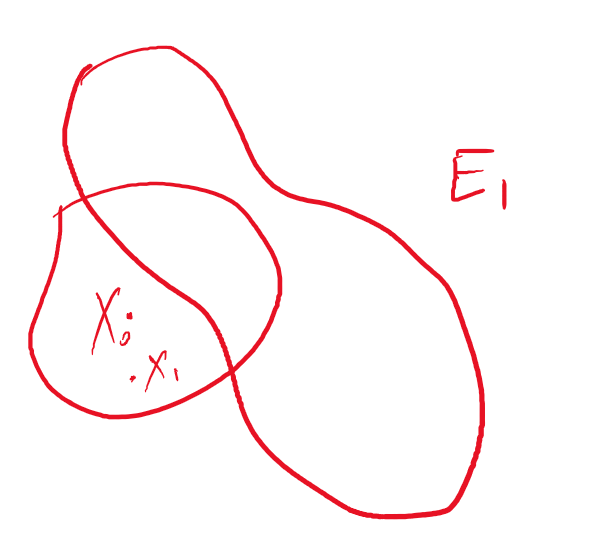
\includegraphics[scale=0.4]{./fig/2.1.4_2.png}
\end{figure}
\[\text{取}x_1 \in B_{r_0}(x_0)-\bar{E}_1=B_{r_0}(x_0)\cap\bar{E}_1^c\text{是个开集,则}\exists \, r_1>0 \ , \quad s.t. \quad B_{2r_1}(x_1) \subset B_{r_0}(x_0)-\bar{E}_1\]
\[\Rightarrow \ \bar{B}_{r_1}(x_1) \subset B_{2r_1}(x_1) \subset B_{r_0}(x_0)-\bar{E}_1\]
\[\text{由于}\bar{E}_2\text{也是疏集} \ , \ B_{r_1}(x_1) \nsubseteq \bar{E}_2\text{则}\exists \, r_2>0 \ , \quad s.t. \quad B_{2r_2}(x_2) \subset B_{r_1}(x_1)-\bar{E}_2\]
\[\Rightarrow \ \bar{B}_{r_2}(x_2) \subset B_{2r_2}(x_2)\cap(\bar{E}_1\cup\bar{E}_2)^c \qquad (\bar{B}_{r_2}(x_2) \subset \bar{B}_{r_1}(x_1) \ and \ \bar{B}_{r_2}(x_2)\cap(\bar{E}_1\cup\bar{E}_2)=\varnothing)\]
由归纳得存在一系列闭球$\{\bar{B}_{r_n}(x_n)\}_{n=1}^{\infty}$
\[s.t. \ \bar{B}_{r_1}(x_1) \supset \bar{B}_{r_2}(x_2) \supset \bar{B}_{r_3}(x_3) \supset \cdots \quad and \quad \bar{B}_{r_n}(x_n)\subset(\bar{E}_1\cup\bar{E}_2\cup\cdots\cup\bar{E}_n)^c=\bigcap_{i=1}^n\bar{E}_i^c\]
\[\Rightarrow \ \bigcap_{i=1}^{\infty}\bar{B}_{r_i}(x_i) \subset \bigcap_{i=1}^{\infty}\bar{E}_i^c=\left(\bigcup_{i=1}^{\infty}\bar{E}_i\right)^c=X^c=\varnothing \quad \text{推出矛盾,故假设不成立}\]
Q.E.D

\subsection{距离空间的完备化与压缩映射} \label{zip}
\paragraph*{例} \quad $S=(C[0,1],d_1) \subset (L^1[0,1],d_1) \ $,$ \ C[0,1]$在$L^1[0,1]$中稠密,称$L^1[0,1]$是$C[0,1]$完备化。\\
\textbf{Proof:}
\[\text{令}x \in L^1[0,1]\text{可积} \ \Leftrightarrow \ \int_0^1|x(t)|dt<+\infty\]
\[\int_0^1|x(t)|dt=\sum_{n=0}^{+\infty} \ \int\limits_{[0,1]\cap\{n \leq |x| \leq n+1\}}|x(t)|dt<+\infty \]
\[ \Rightarrow \ \exists \, N>0 \quad s.t. \quad n \geq N \ , \ \int\limits_{[0,1]\cap\{|x|>N\}}|x(t)|dt<\frac{1}{n}\]
令
\[\tilde{x}(t)=\left \{
\begin{array}{ll}
    x(t) & , x \leq N \\ 0 & , x>N
\end{array}    
\right .\]
由$Lusin$定理,存在连续函数$g_n(t)$,满足
\[m([0,1]/\{\tilde{x}(t)=g_n(t)\})<\frac{1}{nN}\]
\[d_1(g_n(t),x(t)) \leq d_1(g_n(t),\tilde{x}(t))+d_1(\tilde{x}(t),x(t))=\int_0^1|g_n(t)-\tilde{x}(t)|dt+\int_0^1|\tilde{x}(t)-x(t)|dt\]
\[\leq \frac{1}{nN} \cdot N+\int\limits_{[0,1]\cap\{|x(t)|>N\}}|x(t)|dt=\frac{1}{n}+\frac{1}{n}=\frac{2}{n}\]
\[\Rightarrow \ d_1(g_n(t),x(t)) \to 0 \ (n \to \infty)\]
\textbf{Q.E.D.}
\begin{theorem}[$Lusin$定理]
    设$A \in \mathscr{L} \ , \ m(A)<+\infty \ , \ f:A \to \mathbb{R}$是处处有限的$Lebesgue$可测函数,则
    \[\forall \varepsilon>0 \ , \ \exists \, g \in C(A):A\to \mathbb{R} \ , \quad s.t. \quad m(\{g \neq f\}) \leq \varepsilon\]
\end{theorem}
$Lusin$定理实际上表明连续函数和可测函数没太大的差别。

下面我们来介绍一个极其破防的定理以及它更加破防的证明。
\begin{theorem}[完备化定理]
    设$(X,d)$是距离空间,则存在$(\tilde{X},\tilde{d})$是完备距离空间,以及等距映射$F:(X,d) \rightarrow (\tilde{X},\tilde{d})$,且$F(x) \subset (\tilde{X},\tilde{d})$是稠密的。
    称$(\tilde{X},\tilde{d})$是$(X,d)$的完备化。若$(\tilde{Y},\tilde{d}_Y)$是另一个完备化,那么$(\tilde{X},\tilde{d})$与$(\tilde{Y},\tilde{d}_Y)$等距(等距意义下的唯一)。
\end{theorem}
\textbf{Proof:}($\mathbb{Q} \to \mathbb{R}$类似,补全$\mathbb{Q}$中所有柯西列的极限)\\
\textbf{Claim 1 等价类$[\{x_n\}]$}\\
考虑X中所有柯西列的集合,我们称$[\{x_n\}]$和$[\{y_n\}]$等价,如果其满足:
\[\lim_{x \to \infty}d(x_n,y_n)=0 \quad \text{(收敛到同一个点认为是同一类极限)}\]
我们令$\tilde{X}=\{\tilde{x}=[\{x_n\}],\{x_n\}\text{是}X\text{中的柯西列}\} \ $,$ \ [ \quad ]$表示等价类;定义距离
\[\tilde{d}(\tilde{x},\tilde{y})=\lim_{n \to \infty}d(x_n,y_n)\]
下面,我们要证明三件事:1、极限存在;2、$\tilde{d}$的取值与代表元素$x_n,y_n$无关;3、$\tilde{d}$为距离。

1、
\[|d(x_n,y_n)-d(x_m,y_m)| \leq d(x_n,x_m)+d(y_n,y_m)\]
\[\Rightarrow \ \{d(x_n,y_n)\}_{n=1}^{\infty}\text{是}\mathbb{R}\text{中的柯西列} \ \Rightarrow \ \text{收敛} \ \Rightarrow \ \text{该极限存在}\]

2、
\[|d(\tilde{x}_n,\tilde{y}_n)-d(x_n,y_n)| \leq d(\tilde{x}_n,x_n)+d(\tilde{y}_n,y_n)\to 0 \quad (n \to \infty)\]
\[\text{即$\tilde{d}$的收敛性与$[\{x_n\}]$和$[\{x_n\}]$的选取无关}\]

3、
\[\tilde{d}(\tilde{x},\tilde{y})=\lim_{n \to \infty}d(x_n,y_n) \leq \lim_{n \to \infty}d(x_n,z_n)+\lim_{n \to \infty}d(z_n,y_n)=\tilde{d}(\tilde{x},\tilde{z})+\tilde{d}(\tilde{z},\tilde{y})\]
\textbf{Claim 2 $(\tilde{X},\tilde{d})$是完备的}\\
\[\text{设}\{\tilde{x}_n\}\text{是}\tilde{X}\text{中的柯西列,对}\forall \tilde{x} \in \tilde{X}\text{可取代表元}\{x_n\}\text{满足}d(x_n,x_m)\leq \frac{1}{2^k} \ , \ (n,m \geq k)\]
\[(\forall k \ , \ \exists \, n_k>k \ , \quad s.t. \quad n,m \geq n_k \ , \ d(x_n,x_m)<\frac{1}{2^k} \ , \ \text{选取}n_{k+1}>n_k \ , \ \text{则子列}\{x_n\}\text{满足要求})\]
记$\tilde{x}_n=[\{x_{n_i}\}_{i=1}^{\infty}]$,那么我们剩下的事情就是证明任取一个$X$中的柯西列$\{x_n\}$都可以收敛到$\tilde{x}_n$,考虑任取的柯西列的子列$\{x_{n_n}\}$,我们要证明它也是柯西列
\[d(x_{n_n},x_{m_m}) \leq d(x_{n_n},x_{n_m})+d(x_{n_m},x_{m_m}) \leq \frac{1}{2^n}+d(x_{n_m},x_{m_m}) \quad (m>n)\]
其中,对$d(x_{n_m},x_{m_m})$:
\[\forall k \ , \ \exists \, n_k>k \ , \quad s.t. \quad n,m \geq n_k \ , \ \tilde{d}(\tilde{x}_n,\tilde{x}_m)=\lim_{i \to \infty}d(x_{n_i},x_{m_i})<\frac{1}{2^k}\]
\[\Rightarrow \ \exists \, I_k>0 \quad s.t. \quad i \geq I_k \ , \ d(x_{n_i},x_{m_i})<\frac{1}{2^k}\]
\[\Rightarrow \ d(x_{n_m},x_{m_m}) \leq d(x_{n_m},x_{n_{I_k}})+d(x_{n_{I_k}},x_{m_{I_k}})+d(x_{m_{I_k}},x_{m_m}) \leq \frac{1}{2^m}+\frac{1}{2^k}+\frac{1}{2^m} \leq \frac{3}{2^k}\]
\[\Rightarrow \ m,n \geq n_k \ , \ d(x_{n_n},x_{m_m}) \leq \frac{4}{2^k} \ \Rightarrow \ \{x_{n_n}\}\text{为}X\text{中的柯西列}\]
记$\tilde{x}=[\{x_{n_n}\}_{n=1}^{\infty}]$,我们想证明$\tilde{d}(\tilde{x}_n,\tilde{x}) \to 0$
\[\tilde{d}(\tilde{x}_n,\tilde{x})=\lim_{i \to \infty}d(x_{n_i},x_{i_i}) \leq \lim_{i \to \infty}d(x_{n_i},x_{n_n})+\lim_{i \to \infty}d(x_{n_n},x_{i_i}) \leq \frac{1}{2^n}+\frac{1}{2^n}=\frac{2}{2^n}\]
\[\Rightarrow \ \tilde{d}(\tilde{x}_n,\tilde{x}) \to 0 \quad (n \to \infty)\]
\textbf{Claim 3 映射$F:(X,d) \rightarrow (\tilde{X},\tilde{d})$是等距映射,且$F(x) \subset (\tilde{X},\tilde{d})$是稠密的}\\
我们这里定义映射$F$
\[F:(X,d) \to (\tilde{X},\tilde{d}) \quad x \mapsto \tilde{x}=\{x,x,x,\cdots\}\]
$F$是等距映射
\[\tilde{d}(F(x),F(y))=\lim_{n \to \infty}d(\tilde{x},\tilde{y})=d(x,y)\]
记
\[\tilde{x}=[\{x_n\}_{n=1}^{\infty}] \in \tilde{X} \ , \ \tilde{k}_n=\{x_n,x_n,\cdots\} \in F(X)\]
对于$F(x)$的稠密性,我们只需证明,$\forall \tilde{x} \in \tilde{X} \ , \ \exists \, \tilde{k}_n \in F(X) \ , \quad s.t. \quad \tilde{d}(\tilde{k}_n,\tilde{x}) \to 0 \ (n \to \infty)$
\[\tilde{d}(\tilde{k}_n,\tilde{x})=\lim_{i \to \infty}d(k_{n_i},x_i)=\lim_{i \to \infty}d(x_n,x_i) \leq \frac{1}{2^n} \ \Rightarrow \ \tilde{d}(\tilde{k}_n,\tilde{x}) \to 0 \quad (n \to \infty)\]

至此,我们完成了完备化定理存在性部分的证明,我们构造了一个(类)完备距离空间$(\tilde{X},\tilde{d})$,并指出了从原空间$(X,d)$到完备距离空间$(\tilde{X},\tilde{d})$的映射为等距映射,还顺便证明了在等价类意义下,$(X,d)$到$(\tilde{X},\tilde{d})$的映射$F$是一个单射,也即到$(\tilde{X},\tilde{d})$的一个子空间$F(X)$的映射$F$是一个双射。下证唯一性。\\
\textbf{Claim 4 等距意义下的唯一性}\\
设$(\tilde{Y},\tilde{d}_Y)$是$X$的另一个完备化,定义$G:\tilde{Y} \to \tilde{X} \quad y \mapsto [\{x_n\}]$其中$\{x_n\}$是$X$中的一个柯西列,满足
\[\tilde{d}_Y(x_n,y) \to 0 \quad (n \to \infty)\]
因为$\tilde{Y}$,$\tilde{X}$是完备的,故任意给定两个$X$中的柯西列在$\tilde{Y}$,$\tilde{X}$中都能找到对应的像,分别记作$y_1,y_2$和$[\{x_n\}_1],[\{x_n\}_2]$,则
\[\tilde{d}_Y(G(y_1),G(y_2))=\tilde{d}_Y([\{x_n\}_1],[\{x_n\}_2])=\lim_{n \to \infty}\tilde{d}_Y(x_{n_1},x_{n_2})=\tilde{d}_Y(y_1,y_2)\]
即$G$为等距映射(是单射)。\\
\textbf{Q.E.D.}

唯一性证明的部分是想证明所有完备化的距离空间在等距意义下唯一,可以说是想证明等距映射的复合还是等距映射,放到本定理的证明中就是证明$F_x=G \circ F_y$。
\newpage
在完备空间上我们可以定义压缩映射:
\begin{definition}[压缩映射]
    设$(X,d)$是距离空间。若有一映射$T:X \to X$满足
    \[\exists \, \theta \in (0,1) \quad s.t. \quad \forall x,y \in X \ , \ d(T(x),T(y)) \leq \theta d(x,y)\]
    则称$T$为压缩映射。
\end{definition}
\begin{definition}[不动点]
    若$T(x)=x$则称$x$为$T$的不动点。
\end{definition}
\begin{theorem}[压缩映射原理]
    设$(X,d)$是完备距离空间,压缩映射$T:X \to X$,那么$T$有唯一不动点。
\end{theorem}
\textbf{Proof:}\\
\textbf{Claim 1 设$T$是压缩映射(这里不要求完备),$x \in X \ , \ \{T^n(x)\}_{n=0}^{\infty}$是柯西列}\\
(\textbf{Proof:}设$m>n$,
\[d(T^n(x),T^m(x)) \leq \sum_{i=0}^{m-n-1}d(T^{n+i}(x),T^{n+i+1}(x)) \leq \sum_{i=0}^{m-n-1}\theta^{n+i}d(x,T(x))\]
\[=\theta^nd(x,T(x))\sum_{i=0}^{m-n-1}\theta^i=\frac{\theta^n(1-\theta^{m-n})}{1-\theta}d(x,T(x)) < \frac{\theta^n}{1-\theta}d(x,T(x))\]
\[\forall \varepsilon>0 \ , \ \exists \, N>0 \ , \quad s.t. \quad n>N \ , \ \theta^n<\frac{(1-\theta)\varepsilon}{d(x,T(x))} \ \Rightarrow \ \forall m,n \geq N \ , \ d(T^n(x),T^m(x))<\varepsilon\]
)\\
\textbf{存在性}
\[\{T^n(x)\}_{n=0}^{\infty}\text{是柯西列,}X\text{完备} \ \Rightarrow \ \exists \, x_{\infty} \in X \ , \ d(T^n(x),x_{\infty}) \to 0\]
\[T^n(x)=T\left(T^{n-1}(x)\right) \ (n \to \infty) \ \Rightarrow \ x_{\infty}=T(x_{\infty}) \quad (\text{需要}T\text{连续,容易证明})\]
\[\text{上一小步完整证明:}x_{\infty}=\lim_{n \to \infty}T^n(x)=\lim_{n \to \infty}T(T^{n-1}(x))=T(\lim_{n \to \infty}T^{n-1}(x))=T(x_{\infty})\]
\textbf{唯一性}
\[\text{设}T(x)=x \ , \ T(y)=y\]
\[d(x,y)=d(T(x),T(y)) \leq \theta d(x,y) \ \Rightarrow \ d(x,y)=0\]
\begin{proposition}[推广的压缩映射原理]
    设$(X,d)$是完备距离空间,$T:X \to X$满足
    \[\exists \, n_0 \in \mathbb{Z} \ , \ \theta \in (0,1) \ , \quad s.t. \quad d(T^{n_0}(x),T^{n_0}(y))<\theta d(x,y) \ , \ \forall x,y \in X\]
    则$T$有唯一不动点。(不要求$T$是压缩映射,但$T$复合$n_0$次后是压缩映射)
\end{proposition}
\textbf{Proof:}
\[\exists \, ! \, x \in X \quad s.t. \quad T^{n_0}(x)=x \ \Rightarrow \ T \circ T^{n_0}(x)=T(x) \ \Leftrightarrow \ T^{n_0}(T(x))=T(x) \Rightarrow \ T(x)\text{是}T^{n_0}\text{的不动点}\]
\[\text{由唯一性可得}T(x)=x\]

\textbf{Q.E.D.}

下面我们来看几个压缩映射原理应用的例子(证明方程解的唯一性)。
\paragraph*{例1}
\[\vec{\xi}-A\vec{\xi}=\vec{b} \ (\vec{\xi},\vec{b}\in\mathbb{R}^n \ , \ A=[A]_{n \times n}) \ , \ \text{设}A=\{a_{ij}\}\text{且满足} \ 0<\sum_{i=1}^n\sum_{j=1}^na_{ij}^2<1\]
证明:方程存在唯一解。\\
\[X=\mathbb{R}^n\text{ (完备)} \quad T(\vec{\xi})=A\vec{\xi}+\vec{b} \quad \vec{\xi},\vec{\eta} \in X\]
\[d(\vec{\xi},\vec{\eta})=|T(\vec{\xi})-T(\vec{\eta})|=|A(\vec{\xi}-\vec{\eta})|=\sqrt{\sum_{i=1}^n\left(\sum_{j=1}^na_{ij}(\xi_j-\eta_j)\right)^2}\]
\[\leq \sqrt{\sum_{i=1}^n\left(\sum_{j=1}^na_{ij}\right)^2\left(\sum_{k=1}^n(\xi_k-\eta_k)\right)^2}=\sqrt{\sum_{i=1}^n\sum_{j=1}^na_{ij}^2}|\vec{\xi}-\vec{\eta}|=\theta|\vec{\xi}-\vec{\eta}| \quad (\theta \in (0,1))\]
后续证明略
\paragraph*{例2} \quad $Fredholm$积分方程
\[x(t)=\psi(t)+\lambda\int_a^bK(t,s)x(s)ds \ , \ K(t,s) \in C[a,b] \times [a,b] \ , \ \psi(t) \in C[a,b]\]
证明:当$\lambda$足够小的时候方程有唯一解。\\
\[X=C[a,b]\text{ (完备)} \quad d(x,y)=\mathop {\text{sup}}\limits_{t \in [a,b]}|x(t)-y(t)| \ (x(t),y(t) \in X)\]
\[\text{定义}T:C[a,b] \to C[a,b] \quad T(x(t))=\psi(t)+\lambda\int_a^bK(t,s)x(s)ds\]
\[d(T(x(t)),T(y(t)))=\mathop {\text{sup}}\limits_{t \in [a,b]}|T(x(t))-T(y(t))|=\lambda\mathop {\text{sup}}\limits_{t \in [a,b]}\left|\int_a^bK(t,s)(x(s)-y(s))ds\right|\]
$K(t,s)$在闭区域上连续,可得$K(t,s)$有界。
\[d(T(x(t)),T(y(t))) \leq \lambda\mathop {\text{sup}}\limits_{t \in [a,b]}\int_a^b|K(t,s)||x(s)-y(s)|ds \leq \lambda\mathop {\text{sup}}\limits_{t \in [a,b]}|K(t,s)|d(x,y)(b-a)\]
\[\text{当}\lambda\mathop {\text{sup}}\limits_{t \in [a,b]}|K(t,s)|(b-a)<1\text{时,$T$为压缩映射} \ \Rightarrow \ d(T(x(t)),T(y(t))) \leq \theta d(x,y)\]
后续证明略
\paragraph*{例3} \quad $Volterra$积分方程
\[x(t)=\psi(t)+\lambda\int_a^tK(t,s)x(s)ds \ , \ K(t,s) \in C(([a,b] \times [a,b])\cap\{s<=t\}) \ , \ \psi(t) \in C[a,b]\]
\begin{figure}[htbp]
    \center
    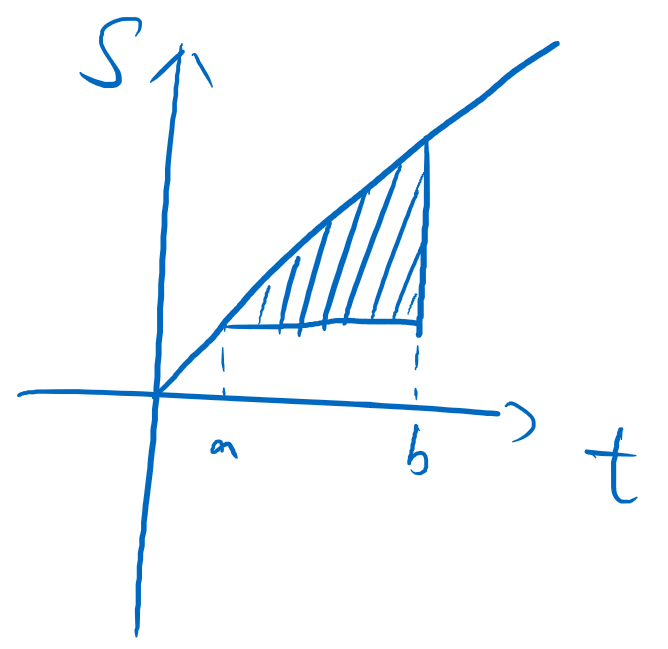
\includegraphics[scale=0.25]{./fig/2.1.5-1.png}
\end{figure}
证明:方程有唯一解。\\
\[T:C[a,b] \to C[a,b] \quad T(x(t))=\psi(t)+\lambda\int_a^tK(t,s)x(s)ds\]
\[d(T(x(t)),T(y(t)))=\lambda\mathop {\text{sup}}\limits_{t \in [a,b]}\left|\int_a^tK(t,s)(x(s)-y(s))ds\right| \leq \lambda\mathop {\text{sup}}\limits_{t \in [a,b]}\left|K(t,s)\right|d(x,y)(t-a)\]
\[d(T^2(x(t)),T^2(y(t)))=\lambda\mathop {\text{sup}}\limits_{t \in [a,b]}\left|\int_a^tK(t,s)\lambda\left|\int_a^tK(t,s)(x(s)-y(s))ds\right|ds\right|\]
\[\leq \lambda^2\left(\mathop {\text{sup}}\limits_{t \in [a,b]}\left|K(t,s)\right|\right)^2d(x,y)\mathop {\text{sup}}\limits_{t \in [a,b]}\left|\int_a^t\int_a^sd\tilde{s}ds\right|\]
\[=\lambda^2\left(\mathop {\text{sup}}\limits_{t \in [a,b]}\left|K(t,s)\right|\right)^2d(x,y)\mathop {\text{sup}}\limits_{t \in [a,b]}\left(\frac{(t-a)^2}{2}\right)=\lambda^2\left(\mathop {\text{sup}}\limits_{t \in [a,b]}\left|K(t,s)\right|\right)^2d(x,y) \cdot \frac{(b-a)^2}{2}\]
易得
\[d(T^n(x(t)),T^n(y(t))) \leq \left(\mathop {\text{sup}}\limits_{t \in [a,b]}\left|K(t,s)\right|\right)^n \cdot \frac{\lambda^n(b-a)^n}{n!}d(x,y):=\frac{\lambda^nM^n(b-a)^n}{n!}d(x,y)\]
\[\lim_{n \to \infty}\frac{\lambda^nM^n(b-a)^n}{n!}=0 \ \Rightarrow \ \exists \, n_0 \ , \quad s.t. \quad \theta=\frac{\lambda^{n_0}M^{n_0}(b-a)^{n_0}}{{n_0}!}<1 \ \Rightarrow \ T^{n_0}\text{是压缩映射}\]
后续证明略
\paragraph*{例extra} \quad $C[a,b]$的完备性 \\
一般来说$C[a,b]$默认的距离应该是
\[d(x,y)=\mathop {\text{sup}}\limits_{t \in [a,b]}|x(t)-y(t)|\]
我们设$\{x_n(t)\}_{i=1}^{\infty}$是柯西列:
\[\forall t \in [a,b] \ , \ \forall \varepsilon>0 \ , \ \exists \, N>0 \ , \ s.t. \forall m,n \geq N \ , \ d(x_n(t),x_m(t))<\varepsilon\]
\[\Leftrightarrow \ \forall t \in [a,b] \ , \ \forall \varepsilon>0 \ , \ \exists \, N>0 \ , \ s.t. \forall m,n \geq N \ , \ |x_n(t)-x_m(t)|<\varepsilon \tag{*}\]
即$x_n(t) \xrightarrow{\text{逐点}} x(t)$
\[\text{令(*)式中 }m \to \infty \ , \ \forall \varepsilon>0 \ , \ \exists \, N>0 \ , \quad s.t. \quad \forall n \geq N \ , \ |x_n(t)-x(t)|<\varepsilon\]
即$x_n(t) \rightrightarrows x(t)$(连续函数一致收敛到连续函数上)
\paragraph*{例4}
\[\left\{
\begin{array}{c}
    \frac{\partial}{\partial t}f(x,t)=\Delta f(x,t)+G(f(x,y)) \quad x \in \mathbb{R}^n \ , \ t \in [0,+\infty) \\
    f(x,0)=\phi(x)
\end{array}
\right.\]
\[\text{设}\phi(x),G(s)\text{有界连续},G(s)\text{在}\mathbb{R}\text{上} 𝐿𝑖𝑝𝑠𝑐ℎ𝑖𝑡𝑧 \text{连续,即}|G(a)-G(b)| \leq L|a,b| \ \forall a,b \in \mathbb{R}\]
令
\[f_0(x,t)=\int_{\mathbb{R}^n}H(x,y,t)\phi(y)dy\]
热方程的解$=$热核$*$(卷)上初始条件。热核:
\[H(x,y,t)=\frac{1}{(4 \pi t)^{\frac{n}{2}}}e^{-\frac{|x-y|^2}{4t}}\]
满足
\[\frac{\partial}{\partial t}f_0=\Delta f_0 \quad \eval{f_0(x,t)}_{t=0}=\phi(x)\]
令
\[T(f(x,t))=f_0(x,t)+\int_0^t\int_{\mathbb{R}^n}H(x,y,t-s)G(f(y,s))dyds\]
后面老师没讲我不会了(寄)。

\section{拓扑空间$Topological \ Space$} \label{topo}
\subsection{真·拓扑空间不完全简介}
在距离空间中,我们是通过距离这个概念引入了开球、开集等集合概念与距离空间中的收敛这个概念,由开球和开集进而导出连续性、紧性;由收敛性我们给出完备性的概念。
\begin{figure}[htbp]
    \center
    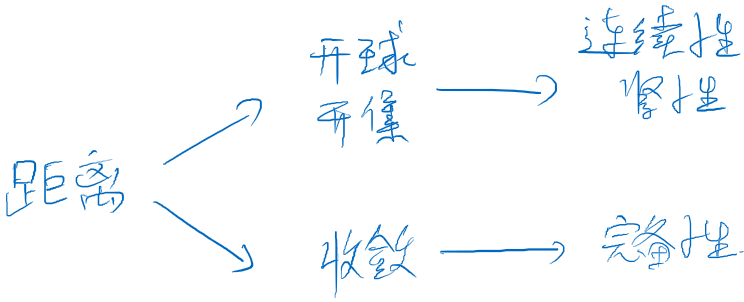
\includegraphics[scale=0.4]{./fig/2.2.1.png}
\end{figure}
但实际上,我们知道(可能不知道)连续性、紧性不一定需要由距离这个概念诱导得到,定义他们只需要开集。

以及在收敛中,我们也发现了弱收敛、逐点收敛并不具有距离概念。

显然距离空间并不是一个足够广泛的空间可以支撑得起这些概念,因此,我们需要考虑一个更广泛的空间,这里我们讲简要介绍拓扑空间。
\begin{definition}[拓扑]
    设$X \neq \varnothing$,记$P(X)=\{X\text{的所有子集}\}$,设$\tau \in P(X)$满足:\\
    \textbf{1.} $\varnothing,X \in \tau$; \qquad \textbf{2.} $\tau$中任意个集合的并属于$\tau$; \qquad \textbf{3.} $\tau$中有限个集合的交属于$\tau$。\\
    则称$\tau$是$X$上的拓扑,$\tau$中的集合称为开集。(拓扑就是指定集合上的哪些子集是开集)
\end{definition}
\paragraph*{例1} $(X,d)$是距离空间,$\tau_d=\{x\text{中的开集}\}$
\paragraph*{例2} $X=\{0,1\}$,令
\[\tau_1=\{\varnothing,X\}\text{(平凡拓扑)} \quad \tau_2=\{\varnothing,\{0\},X\}\text{(是个拓扑)}\]
\[\tau_3=\{\varnothing,\{0\},\{1\},X\}\text{(离散拓扑,由$X$的所有子集组成的拓扑,包含$X$的所有单点集)}\]

若在$X$上,$\tau_1 \subset \tau_2$,则称$\tau_2$强于$\tau_1$。
\begin{definition}[闭集]
    若$A^c \in \tau$,则称$A$是闭集。($A$是闭集$\ \Leftrightarrow \ A=\bar{A}$)
\end{definition}
\begin{definition}[邻域]
    设$x \in X \ , \ U_x \subset \tau \ , \ x \in U_x$,则称$U_x$是$x$的一个邻域(包含$x$的开集)
\end{definition}
\begin{definition}[连续]
    定义$f:X \to Y$是拓扑空间到拓扑空间的映射,设$x_0 \in X$,若对任意$f(x_0)$的邻域$V_{f(x_0)}$都存在$X$中$x_0$的邻域$U_{x_0}$使得$f(U_{x_0}) \subset V_{f(x_0)}$,则$f$称在$x_0$处连续。
\end{definition}
\begin{theorem}
    若$X,Y$是拓扑空间,$f:X \to Y$是连续映射当且仅当开集的原像是开集。
\end{theorem}
这里我们规定符号$f^{-1}$仅表示原像
\[f:X \to Y \ (A \subseteq Y) \quad f^{-1}(A)=\{x \in X \ , \ f(x) \in A\}\]
最后给个奇怪的例子作为这一小节的总结,在下一小节虽然我们也将介绍一些拓扑空间中可以定义的概念,但我们更愿意将他放到距离空间的背景下来考量,因为这门课是泛函分析(乐)。
\paragraph*{奇怪的例子} 定义如下拓扑

$X=\{0,1\} \quad \tau_D=\{\varnothing,\{0\},\{1\},X\}$单点集在$\mathbb{R}^n$和距离空间中是闭集,但这里是开集。

\subsection{紧集}
在介绍距离空间上的紧性之前,我们需要介绍一下四种分离公理并指认距离空间所属的公理。
\begin{proposition}[分离公理]
    $T_1$公理:$\forall x \neq y \ , \ \exists \, U_x,U_y \ , \quad s.t. \quad x \in U_x \ , \ y \notin U_x \ ; \ y \in U_y \ , \ x \notin U_y$\\
    $T_2$公理:$\forall x \neq y \ , \ \exists \, U_x \cap U_y=\varnothing \ , \quad s.t. \quad x \in U_x \ , \ y \notin U_x \ ; \ y \in U_y \ , \ x \notin U_y$\\
    $T_3$公理:$\forall$ 闭集$A \cap x=\varnothing \ , \ \exists \, U_x \cap U_A=\varnothing \ , \quad s.t. \quad x \in U_x \ , \ A \notin U_x \ ; \ A \in U_A \ , \ x \notin U_A$\\
    $T_4$公理:$\forall$ 闭集$A \cap B=\varnothing \ , \ \exists \, U_A \cap U_B=\varnothing \ , \quad s.t. \quad A \in U_A \ , \ B \notin U_A \ ; \ B \in U_B \ , \ B \notin U_A$
\end{proposition}
很显然,这四个公理的限制逐级加强,下面我们可以来看看这几个公理的形象化描述:
\begin{figure}[htbp]
    \center
    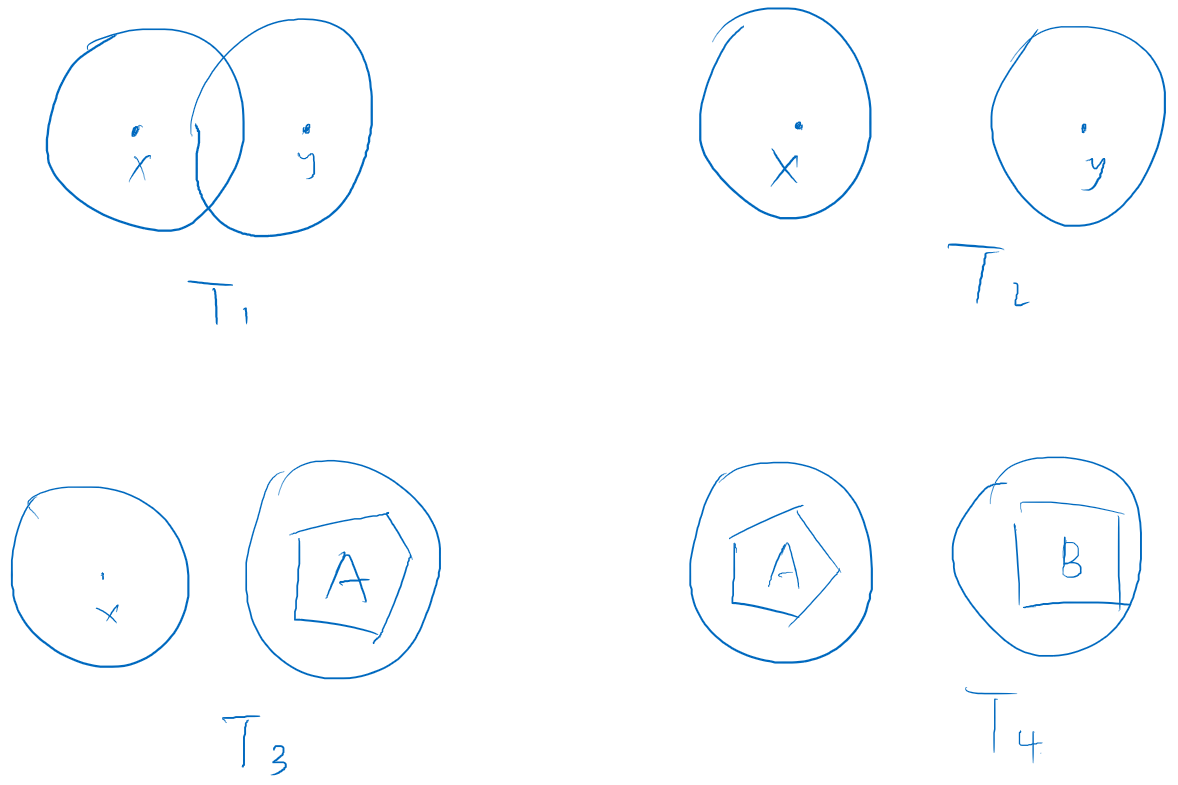
\includegraphics[scale=0.4]{./fig/2.2.2.png}
\end{figure}
对应$T_2$公理,我们又将其称为$Hausdorff$性质,距离空间是满足$T_4$公理的,对于这件事我们可以来证明一下。
\begin{theorem}
    距离空间满足$T_4$公理。
\end{theorem}
Proof(反证法):先预设一些对象:
\[\bar{A}=A \ , \ \bar{B}=B \ , \ A \cap B=\varnothing \ , \ f_A(x):=\mathop {\text{inf}}\limits_{y \in A}d(x,y) \ , \ f_B(x):=\mathop {\text{inf}}\limits_{y \in B}d(x,y)\]
\textbf{Claim} \quad $f_A(x)>0 \ \Rightarrow \ x \notin A$\\
(\textbf{Proof:}反证法

若$f_A(x)=0 \ \Rightarrow \ \exists \, \{y_n\} \subset A \quad s.t. \quad d(x,y_n) \to 0 \ \Rightarrow \ x$是$A$的接触点$ \ \Rightarrow \ x \in \bar{A}=A$\\
矛盾)\\
记
\[U_B=\bigcup_{x \in B}B_{\frac{1}{2}f_A(x)}(x) \ , \ B \subset U_B \qquad U_A=\bigcup_{x \in A}B_{\frac{1}{2}f_B(x)}(x) \ , \ A \subset U_A \quad \text{都是开集}\]
假设
\[\exists \, z \in U_A \cap U_B \ \Rightarrow \ \exists \, x \in A \quad s.t. \quad z \in B_{\frac{1}{2}f_B(x)}(x) \ , \ \exists \, y \in B \quad s.t. \quad z \in B_{\frac{1}{2}f_A(y)}(y)\]
\[\Rightarrow \ d(x,z)<\frac{1}{2}f_B(x) \ , \ d(z,y)<\frac{1}{2}f_A(y)\]
\[d(x,y) \leq d(x,z)+d(z,y)<\frac{1}{2}f_B(x)+\frac{1}{2}f_A(y)<\frac{1}{2}d(x,y)+\frac{1}{2}d(x,y)=d(x,y)\]
矛盾。
\begin{definition}[子集拓扑]
    $(X,\tau)$为拓扑空间,$A \subset X$,令$\tau_A=\{U \cap A \ , \ U \in \tau\}$,则称$\tau_A$为$X$上的子集拓扑(诱导拓扑)。
\end{definition}
下面,我们将要开始引入我们我们这小节的主要内容,刻画距离空间的紧性,接着上面的内容,我们先看看拓扑空间下紧性的定义。
\begin{definition}[紧(致)性]
    $(X,\tau)$为拓扑空间,若$X$的任意开覆盖都有有限子覆盖,则称$X$是紧(致)的。
    \[X \subset \bigcup_{\lambda \in \Lambda}A_{\lambda} \ \text{$A_{\lambda}$是开集} \ \Rightarrow \ X \subset \bigcup_{i=1}^kA_{\lambda_i}\]
\end{definition}
\paragraph*{例} $\mathbb{R}^n$上的闭区间(有界闭集)是紧的。
\begin{definition}[紧集]
    $(X,\tau)$为拓扑空间,$A \subset (X,\tau)$,若$(A,\tau_A)$是紧的,则称$A$是$X$中的紧集。
\end{definition}
下面我们将讨论拓扑空间下闭集和紧集的关系,我们知道欧氏空间中紧集就是有界闭集,那么这个性质在一般的拓扑空间中还成立吗?
\begin{theorem}
    紧空间的闭子集一定是紧集。
\end{theorem}
\textbf{Proof:}设$X$是一紧空间(或者拓扑空间中的紧子集),$A \subset X$,设
\[A \subset \bigcup_{\lambda \in \Lambda}U_{\lambda} \ \Rightarrow \ X \subset \left(\bigcup_{\lambda \in \Lambda}U_{\lambda}\right) \cup A^c\]
因为$X$是紧的,有
\[\exists \, \lambda_1,\lambda_2,\cdots,\lambda_k>0 \quad s.t. \quad X \subset \left(\bigcup_{i=1}^kU_{\lambda_i}\right) \cup A^c\]
\[A \subset X \subset \left(\bigcup_{i=1}^kU_{\lambda_i}\right) \cup A^c\]
故$A$是紧的。\\
\textbf{Q.E.D.}
\begin{theorem}
    $T_2$空间的紧子集是闭集。
\end{theorem}
\textbf{Proof:}设$X$是$T_2$空间,$A \subset X$,需证明$A^c$为开集,即需证$\forall x \in A^c \ , \ \exists \, U_x \subset A^c$。

设$y \in A \ , \ x \in A^c$,由$T_2$公理,存在$x$的开邻域$U_{x,y}$,$y$的开邻域$V_{x,y}$($U_{x,y},V_{x,y}$选取与$x,y$都有关)满足$U_{x,y} \cap V_{x,y}=\varnothing$
\[\Rightarrow \ A \subset \bigcup_{y \in A}V_{x,y} \ , \ \text{由紧性} \ , \ \exists \, y_1,y_2,\cdots,y_k \in A \quad s.t. \quad A \subset \bigcup_{i=1}^kV_{x,y_i}\]
\[\text{令}U_x=\bigcup_{i=1}^kU_{x,y_i} \ \Rightarrow \ U_x \cap \bigcup_{i=1}^kV_{x,y_i}=\varnothing \ \Rightarrow \ U_x \cap A=\varnothing \ \text{即} \ U_x \cap A^c\]
\textbf{Q.E.D.}

可以看到,在一般拓扑空间下紧和闭是两个等同的概念,紧比闭更强一点。下面我们来看一个紧的性质结束这一小节。
\begin{theorem}
    紧空间(子集)在连续映射下的像也是紧的。
\end{theorem}
\textbf{Proof:}
\begin{figure}[htbp]
    \center
    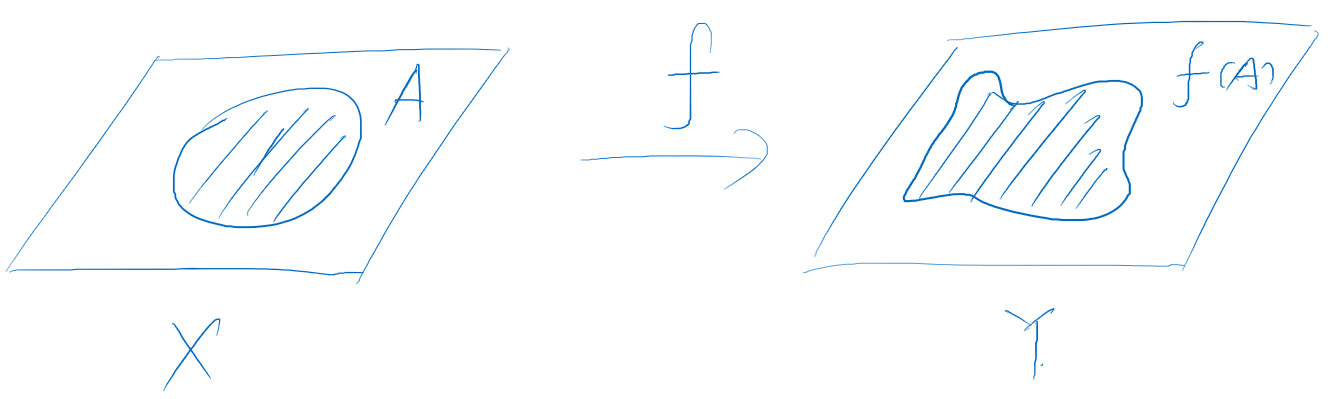
\includegraphics[scale=0.2]{./fig/2.2.2-1.png}
\end{figure}
\[\text{设}A \subset X\text{是紧的,}f(A) \subset \bigcup_\alpha G_\alpha \ , \ \{G_{\alpha}\}\text{为}Y\text{中的一族开集}\]
\[\text{由$f$为连续映射可得}f^{-1}(G_{\alpha})\text{是开集且}A \subset \bigcup_{\alpha}f^{-1}(G_{\alpha})\]
\[\text{由$A$紧可得} \exists \, \alpha_1,\alpha_2,\cdots,\alpha_k \quad s.t. \quad A \subset \bigcup_{i=1}^kf^{-1}(G_{\alpha_1}) \ , \ f(A) \subset \bigcup_{i=1}^kG_{\alpha_i}\]

\textbf{Q.E.D.}

\subsection{刻画距离空间上的紧集} \label{compact}
下面我们来看距离空间中的紧集是如何定义的。
\begin{definition}[距离空间中的紧集]
    $(X,d)$为距离空间,$A \subset X$,
    \[A \subset \bigcup_{\lambda \in \Lambda}B_{r_{\lambda}}(x_{\lambda})\text{是$A$的任一开球覆盖必有一有限子覆盖}\bigcup_{i=1}^kB_{r_{\lambda_i}}(x_{\lambda_i})\]
    则称$A$是$X$中的紧集。
\end{definition}
顺便再额外看一下有界性的定义。
\begin{definition}[距离空间中的有界性]
    $(X,d)$为距离空间,$A \subset X$,
    \[\exists \, R>0 \ , \ x \in X \ , \quad s.t. \quad A \subset B_R(x)\]
    则称$A$有界。
\end{definition}
\paragraph*{例1} $\mathbb{R}^n$上的紧集是有界闭集,但在一般距离空间中不再成立。

\paragraph*{例2} $l^2$空间是完备的,其上的闭球$\bar{B}_1(0)$不是紧集。
\[l^2=\left\{\{x_n\}_{n=1}^{\infty} \ , \ x_n \in \mathbb{R} \ , \ \sum_{n=1}^{\infty}x_n^2<\infty\right\} \quad d(x,y)=\sqrt{\sum_{n=1}^{\infty}(x_n-y_n)^2}\]
\textbf{Proof:}令$x_n=\{0,0,\cdots,1,0,\cdots\}$(第$n$个为$1$) \quad $x_n \in \bar{B}_1(0) \ (d(x_n,0)=\sqrt{1^2}=1)$
\[\forall n \neq m \ , \ d(x_n,x_m)=\sqrt{1^2+1^2}=\sqrt{2} \ \text{当$m,n$足够大的时候并不趋于0} \ \Rightarrow \ \bar{B}_1(0)\text{不是列紧的}\]
在后续的介绍中,我们会证明,度量空间中列紧的闭集就是紧集,所以这里我们就能看出$\bar{B}_1(0)$不是紧集。当然我们需要解释一下什么是列紧。
\begin{definition}[(相对)列紧性]
    若集合$A$中的任意点列都有收敛子列,则称$A$是列紧的,不要求极限也在$A$中(当$A$为闭时,则极限必然在$A$中,但列紧性要求极限在集合中)。
\end{definition}
在上述例子中我们可以看出列紧是比紧更弱一点的条件。下面我们给出一般距离空间和完备距离空间中紧集的完整刻画,并证明他们。
\begin{theorem}
    距离空间中的子集是紧集当且仅当它是列紧的闭集。
\end{theorem}
\textbf{Proof:}(紧$ \ \Rightarrow \ $列紧闭)
\[A \text{是列紧的闭集} \ \Leftrightarrow \ \forall\{y_n\} \subset A\text{都有收敛子列}y_{n_k} \to y \in A\]

反证法:设$\{y_n\} \subset A$,它的任意子列不收敛于$A$中的点。
\[\forall x \in A \ , \ \exists \, r_x>0 \ , \ B_{r_x}(x) \cap \{y_n\}=\{y_{n_1},y_{n_2},\cdots,y_{n_k}\} \ (k<\infty) \ , \ A \subset \bigcup_{x\in A}B_{r_x}(x)\]
由$A$的紧性:
\[\exists \, x_1,x_2,\cdots,x_k \in A \ , \quad s.t. \quad A \subset \bigcup_{i=1}^kB_{r_{x_i}}(x_i) \ \Rightarrow \ A \cap \{y_n\}=\{y_{n_1},y_{n_2},\cdots,y_{n_j}\} \ (j<\infty)\]
推出矛盾。\\
\textbf{Q.E.D.}

另外一半比较难证明,我们需要先引入全有界的概念,然后通过几个引理逐步证明。
\begin{definition}[全有界性]
    $(X,d)$是距离空间,$A \subset X$,
    \[\forall \varepsilon>0 \ , \ \exists \, k<\infty \ , \ x_i \in A \ (i=1,2,\cdots,k) \quad s.t. \quad A \subset \bigcup_{i=1}^kB_{\varepsilon}(x_i) \ (k\text{与$\varepsilon$有关})\]
    则称$A$是全有界的。
\end{definition}
\begin{figure}[htbp]
    \center
    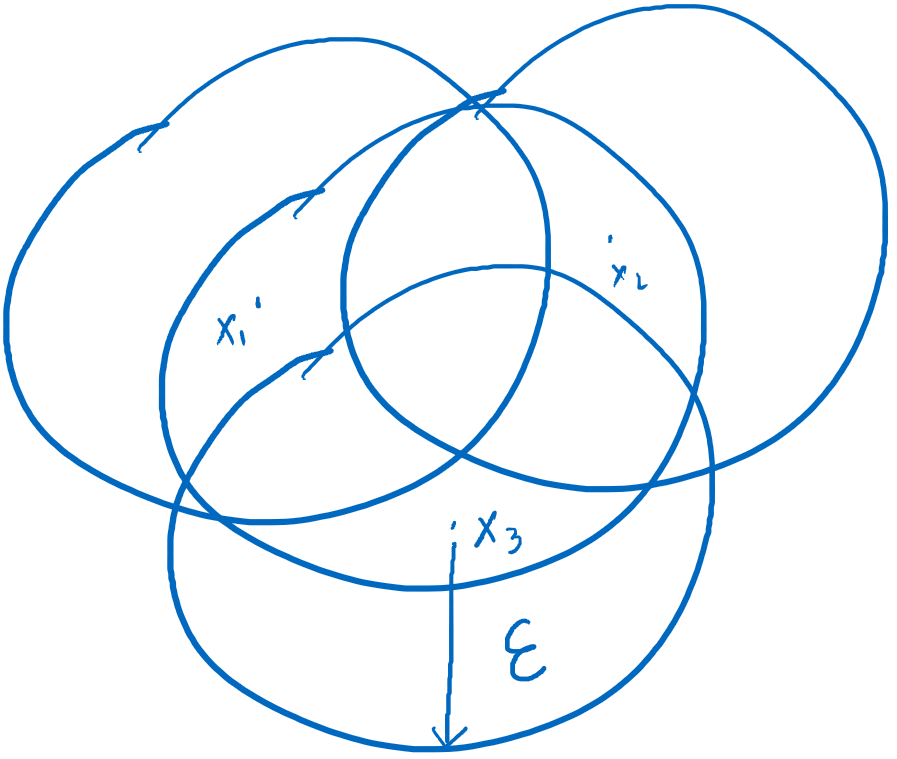
\includegraphics[scale=0.25]{./fig/2.2.3.png}
\end{figure}
显然,全有界集一定是有界集。
\paragraph*{例} \quad $\mathbb{R}^n$中的有界集$\ \Leftrightarrow \ $全有界集。
\begin{definition}[有限$\varepsilon$-网]
    $\{x_i\}_{i=1}^k$称为$A$的有限$\varepsilon$-网。
\end{definition}
接下来我们来证明另外一半:\\
\textbf{Proof:}(列紧闭$ \ \Rightarrow \ $紧)\\
\textbf{Claim 1 全有界集可分}\\
\textbf{Proof:}设$A$为全有界集,对任意$n \in \mathbb{Z}_+$,存在$A$的有限$\varepsilon$-网$B_n$,不妨取$B_n \subset A$
\[\text{考虑}B=\bigcup_{n=1}^{\infty}B_n \ , \ (\text{想证}\bar{B}=A)\]
\[\forall x \in A \ , \ \varepsilon>0 \ , \ \exists \, n_{\varepsilon}=\left[\frac{1}{\varepsilon}\right]+1 \quad s.t. \quad \exists \, y \in B_{n_{\varepsilon}} \ , \ d(x,y)<\frac{1}{n_{\varepsilon}}<\varepsilon\]
\[\Rightarrow \ B_{\varepsilon}(x) \cap B_{n_{\varepsilon}} \neq \varnothing \ \Rightarrow \ B_{\varepsilon}(x) \cap B \neq \varnothing \ \Rightarrow \ x \in \bar{B} \ \Rightarrow \ A \subset \bar{B} \ \Leftrightarrow \ A\text{可分}\]
\textbf{Q.E.D.}\\
\textbf{Claim 2 距离空间中的列紧集是全有界的}\\
\textbf{Proof:}反证:若列紧的$A$不是全有界的,则存在$\varepsilon_n>0$,$A$没有有限$\varepsilon_n$-网。
\[\forall x_0 \in A \ , \ A-B_{\varepsilon_n}(x_0) \neq \varnothing\]
\[\forall x_1 \in A-B_{\varepsilon_n}(x_0) \ , \ A-\bigcup_{i=0}^1B_{\varepsilon_n}(x_i) \neq \varnothing\]
由归纳得存在点列$\{x_n\}_{n=0}^{\infty} \subset A$不收敛$(\forall i \neq j \ , \ d(x_i,x_j)>\varepsilon_n)$,即$A$中点列不全有收敛子列,与题设矛盾。\\
\textbf{Q.E.D.}\\
\textbf{Claim 3 距离空间中的子集是全有界的,那子集的任一开覆盖必有有限子覆盖}\\
\textbf{Proof:}设$A$为全有界集,由引理1可得$A$是可分的,我们设$A$的稠密可数子集为$S$
\[\text{假设有开覆盖}A \subset \bigcup_{\alpha}G_{\alpha} \ , \ \forall x \in A \ , \ \exists \, \alpha \ , \quad s.t. \quad x \in G_{\alpha}(\text{开集}) \ \Rightarrow \ \exists \,r>0 \ , \quad s.t. \quad B_r(x) \subset G_{\alpha}\]
\[B_{\frac{1}{4}r}(x) \cap S \neq \varnothing \ \text{(稠密要求不能有"空洞",不然闭包盖不住全集)} \ \Rightarrow \ y \in B_{\frac{1}{4}r}(x) \cap S\]
\[\text{取}r' \in \left(\frac{r}{4},\frac{r}{2}\right) \cap \mathbb{Q} \ , \ \text{则有} \ x \in B_{r'}(y) \ \text{且} \ B_{r'}(y) \subset B_{r}(x) \subset G_{\alpha}\]
\[\Rightarrow \ A \subset \bigcup_{r' \in \mathbb{Q}}\bigcup_{y \in S}B_{r'(y)}(y) \ \Rightarrow \ A\text{被可数个}B_{r'}(y)\text{覆盖} \ \Rightarrow \ A\text{被可数个}G_{\alpha}\text{覆盖}\]
\textbf{Q.E.D.}\\
下面我们开始正式证明刻画1的另一半:\\
\textbf{Proof (body):}
\[A\text{是列紧闭集,可知}A\text{是全有界的,且其任意开覆盖} \ A \subset \bigcup_{\alpha}G_{\alpha} \ \text{必有可数子覆盖} \ A \subset \bigcup_{i=1}^{\infty}G_{\alpha_i}\]
采用反证法,假设$A$不是紧的,则存在一个$A$的开覆盖无有限子覆盖:
\[\exists \, \{G_{\alpha_i}\}_{i=1}^{\infty} \ , \ \forall n \in \mathbb{Z}_+ \ , \ A \nsubset \bigcup_{i=1}^nG_{\alpha_i} \ \Rightarrow \ \text{取}x_n \in A-\bigcup_{i=1}^nG_{\alpha_i} \ (n=1,2,\cdots)\]
易知,$\forall n \in \mathbb{Z}_+$,$G_{\alpha_n}$中只包含$\{x_n\}$中的有限个点。\\
\[\text{由}A\text{是列紧的闭集可知,} \ \exists \, \{x_{n_k}\}_{k=1}^{\infty} \subset \{x_n\}_{n=1}^{\infty} \ , \quad s.t. \quad \lim_{k \to \infty}x_{n_k}=x \in A\]
\[\Rightarrow \ \exists \, n_0>0 \quad s.t. \quad x \in G_{\alpha_{n_0}} \ \Rightarrow \ \exists \, r>0 \quad s.t. \quad B_r(x) \subset G_{\alpha_{n_0}} \ \Rightarrow \ \exists \, N>0 \quad s.t. \quad k \geq N \ , \ x_{n_k} \in B_r(x)\]
与题设矛盾。\\
\textbf{Q.E.D.}
\begin{theorem}
    完备距离空间中的子集是紧集当且仅当它是全有界闭集。
\end{theorem}
在上一个定理的证明中,我们结合前半部分的证明与后半部分的Claim 2,即证毕该定理的前一半,下面我们只需证明另一部分。其实这里已经可以看出三个条件的强弱:
\[\text{紧}>\text{列紧}>\text{全有界}\]
Proof (完备距离空间中的全有界闭集是紧集):\\
\textbf{Claim 完备距离空间中全有界集是列紧的}\\
\textbf{Proof:}设$A$全有界,$\{x_n\} \subset A$,
\[\exists \, A\text{的有限}1\text{-网}N_1 \ \Rightarrow \ \exists \, x \in N_1 \ , \ B_1(x) \cap \{x_n\}\text{有无限多个点,取其中一个点记作}x_{n_1}\]
\[B_1(x) \cap A\text{也是全有界的} \ , \ \exists \, A\text{的有限}\frac{1}{2}\text{-网}N_2 \ , \ \text{同理取其中一个点记作}x_{n_2}\]
\[\vdots\]
由归纳得
\[\exists \, \{x_{n_k}\}_{k=1}^{\infty} \quad s.t. \quad d(x_{n_k},x_{n_{k+m}})<\frac{1}{2^k} \ \Rightarrow \ \{x_{n_k}\}\text{是柯西列}\]
由完备性,$\exists \, x \in A \quad s.t. \quad x_{n_k} \to x \ , \ (k \to \infty)$。\\
\textbf{Q.E.D.}\\
再由上一个定理后半部分证明的结论可知,距离空间中的列紧闭集是紧集,则证毕。\\
\textbf{Q.E.D.}
\begin{figure}[htbp]
    \center
    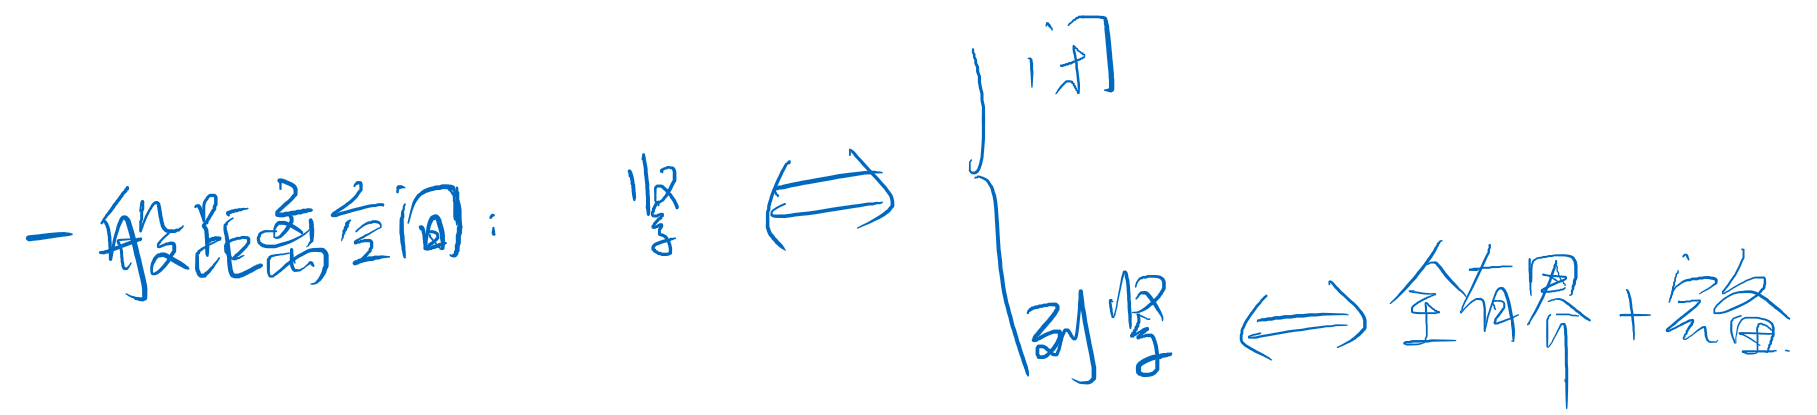
\includegraphics[scale=0.25]{./fig/2.2.3-1.png}
\end{figure}

接下来我们可以看看具体完备距离空间中的(列)紧性的刻画。

\paragraph*{例} \quad $C[a,b]$上的(列)紧性的刻画($Arzela-Ascoli$定理)

为此,我们需要先铺垫一些定义:
\begin{definition}[一致有界]
    $A \subset C[a,b]$,且满足
    \[\exists \, k>0 \ , \ \forall x(t) \in A \ , \ t \in [a,b] \quad s.t. \quad |x(t)| \leq k\]
    则称$A$为一致有界的(与距离空间中的有界是同一回事)。
\end{definition}
\begin{definition}[等度(一致)连续]
    $\forall \varepsilon>0 \ , \ \exists \, \delta>0 \ $,
    \[\forall x(t) \in A \ , \ t_1,t_2 \in [a,b] \ , \ |t_1-t_2|<\delta \quad s.t. \quad |x(t_1)-x(t_2)|<\varepsilon\]
    则称$A$是等度(一致)连续的。
\end{definition}
可以看出,等度(一致)连续是对一族函数的“一致连续”,其$\varepsilon,\delta$的取值与函数无关,容易看出它比一致连续强。

\paragraph*{例1} \quad $\exists \, M>0 \ , \ \forall x(t) \in A \ , \ \forall t \in [a,b] \quad s.t. \quad |x'(t)| \leq M \ $,则$A$是等度连续。\\
\textbf{Proof:}
\[|x(t_1)-x(t_2)|=|x'(\xi)||t_1-t_2| \leq M|t_1-t_2| \quad \xi \in (t_1,t_2) \ : \ |t_1-t_2| \to 0 \ , \ |x(t_1)-x(t_2)| \to 0\]
\textbf{Q.E.D.}

这个命题还能推广,证明也类似。

\paragraph*{例2} \quad $A \subset C^1[a,b]$且$A$在$C^1[a,b]$,则$A$在$C[a,b]$是等度连续。
\begin{theorem}[$Arzela-Ascoli$定理] \label{the:AA}
    $C[a,b]$的子集是列紧的当且仅当它是一致有界且等度连续的。
\end{theorem}
Proof ($C[a,b]$列紧$ \ \Rightarrow \ $全有界$ \ \Rightarrow \ $有界):
\[\forall \varepsilon>0 \ , \ \exists \, A\text{的有限}\frac{\varepsilon}{3}\text{-网}N\text{满足} \ \forall x_i \in N \ , \ \exists \,\delta_i \ , \ t_1,t_2 \in [a,b] \ , \ |t_1-t_2|<\delta_i \quad s.t. \quad |x(t_1)-x(t_2)|<\varepsilon\]
\[\text{取}\delta=\mathop \text{min}\limits_{N}\{\delta_i\} \ , \ \exists \, i \quad s.t. \quad x(t) \subset B_{\frac{\varepsilon}{3}}(x_i(t)) \quad \text{则当}|t_1-t_2|<\delta \ , \ \forall x(t) \in A \ \text{时,有}\]
\[|x(t_1)-x(t_2)| \leq |x(t_1)-x_i(t_1)|+|x_i(t_1)-x_i(t_2)|+|x_i(t_2)-x(t_2)|<\frac{\varepsilon}{3}+\frac{\varepsilon}{3}+\frac{\varepsilon}{3}=\varepsilon\]
\textbf{Q.E.D.}

Proof ($C[a,b]$等度连续,一致有界$ \ \Rightarrow \ $列紧):\\
由于$C[a,b]$完备,故只需证明$C[a,b]$全有界。
\[\forall \varepsilon>0 \ , \ \exists \, \delta>0 \ , \ |t_1-t_2|<\delta \ , \ \forall x(t) \in A \quad s.t. \quad |x(t_1)-x(t_2)|<\varepsilon\]
\[\exists \, k>0 \ , \ \forall x(t) \in A \ , \ t \in [a,b] \quad s.t. \quad |x(t)|<k \quad \text{一致有界}\]
\[\text{取$[-k,k]$划分}:\{y_0,y_1,\cdots,y_n\}:y_0=-k \ , \ y_n=k \ , \ 0<y_{i+1}-y_i<\frac{\varepsilon}{5}\]
\[\text{取$[a,b]$划分}:\{t_0,t_1,\cdots,t_m\}:t_0=a \ , \ t_m=b \ , \ 0<y_{i+1}-y_i<\delta\]
\[\text{若}x(t_i) \in [y_k,y_{k+1}] \ , \ \text{令}f(t_i)=y_k \ , \ \text{其他地方用直线连接,则}\forall t \in [a,b] \ , \ \exists \, t_i \quad s.t. \quad t \in [t_i,t_{i+1}]\]
\begin{figure}[htbp]
    \center
    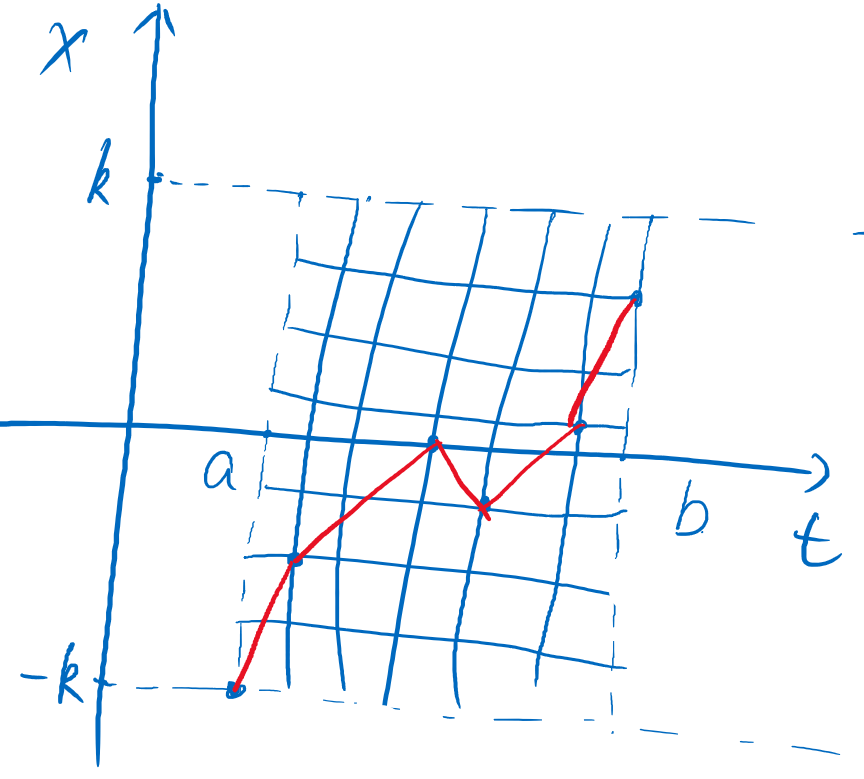
\includegraphics[scale=0.3]{./fig/2.2.3-2.png}
\end{figure}
\[|x(t)-f(t)| \leq |x(t)-x(t_i)|+|x(t_i)-f(t_i)|+|f(t_i)-f(t)|<\frac{\varepsilon}{5}+\frac{\varepsilon}{5}+|f(t_i)-f(t)|\]
\[<\frac{2}{5}\varepsilon+|f(t_i)-f(t_{i+1})|<\frac{2}{5}\varepsilon+|f(t_i)-x(t_i)|+|x(t_i)-x(t_{i+1})|+|x(t_{i+1})-f(t_{i+1})|\]
\[<\frac{2}{5}\varepsilon+\frac{1}{5}\varepsilon+\frac{1}{5}\varepsilon+\frac{1}{5}\varepsilon=\varepsilon\]
\[\text{因$f$至多有限个}(n+1)^{m+1} \ \Rightarrow \ \text{这些$f$构成$A$的一个有限$\varepsilon$-网}\]
\textbf{Q.E.D.}

至此,一般空间的部分我们已经叙述完成,在这一章中我们介绍了距离空间和拓扑空间的一些性质,这些性质将对后续我们叙述具体的距离空间有很大的帮助。